%Input preamble
%Style
\documentclass[12pt]{article}
\usepackage[top=1in, bottom=1in, left=1in, right=1in]{geometry}
\parindent 22pt
\usepackage{fancyhdr}

%Packages
\usepackage{adjustbox}
\usepackage{amsmath}
\usepackage{amsfonts}
\usepackage{amssymb}
\usepackage{bm}
\usepackage[table]{xcolor}
\usepackage{tabu}
\usepackage{color,soul}
\usepackage{makecell}
\usepackage{longtable}
\usepackage{multirow}
\usepackage[normalem]{ulem}
\usepackage{etoolbox}
\usepackage{graphicx}
\usepackage{tabularx}
\usepackage{ragged2e}
\usepackage{booktabs}
\usepackage{caption}
\usepackage{fixltx2e}
\usepackage[para, flushleft]{threeparttablex}
\usepackage[capposition=top,objectset=centering]{floatrow}
\usepackage{subcaption}
\usepackage{pdfpages}
\usepackage{pdflscape}
\usepackage{natbib}
\usepackage{bibunits}
\definecolor{maroon}{HTML}{990012}
\usepackage[colorlinks=true,linkcolor=maroon,citecolor=maroon,urlcolor=maroon,anchorcolor=maroon]{hyperref}
\usepackage{marvosym}
\usepackage{makeidx}
\usepackage{tikz}
\usetikzlibrary{shapes}
\usepackage{setspace}
\usepackage{enumerate}
\usepackage{rotating}
\usepackage{tocloft}
\usepackage{epstopdf}
\usepackage[titletoc]{appendix}
\usepackage{framed}
\usepackage{comment}
\usepackage{xr}
\usepackage{titlesec}
\usepackage{footnote}
\usepackage{longtable}
\newlength{\tablewidth}
\setlength{\tablewidth}{9.3in}
\setcounter{secnumdepth}{4}

\titleformat{\paragraph}
{\normalfont\normalsize\bfseries}{\theparagraph}{1em}{}
\titlespacing*{\paragraph}
{0pt}{3.25ex plus 1ex minus .2ex}{1.5ex plus .2ex}
\makeatletter
\pretocmd\start@align
{%
  \let\everycr\CT@everycr
  \CT@start
}{}{}
\apptocmd{\endalign}{\CT@end}{}{}
\makeatother
%Watermark
\usepackage[printwatermark]{xwatermark}
\usepackage{lipsum}
\definecolor{lightgray}{RGB}{220,220,220}
%\newwatermark[allpages,color=lightgray,angle=45,scale=3,xpos=0,ypos=0]{Preliminary Draft}

%Further subsection level
\usepackage{titlesec}
\setcounter{secnumdepth}{4}
\titleformat{\paragraph}
{\normalfont\normalsize\bfseries}{\theparagraph}{1em}{}
\titlespacing*{\paragraph}
{0pt}{3.25ex plus 1ex minus .2ex}{1.5ex plus .2ex}

\setcounter{secnumdepth}{5}
\titleformat{\subparagraph}
{\normalfont\normalsize\bfseries}{\thesubparagraph}{1em}{}
\titlespacing*{\subparagraph}
{0pt}{3.25ex plus 1ex minus .2ex}{1.5ex plus .2ex}

%Functions
\DeclareMathOperator{\cov}{Cov}
\DeclareMathOperator{\corr}{Corr}
\DeclareMathOperator{\var}{Var}
\DeclareMathOperator{\plim}{plim}
\DeclareMathOperator*{\argmin}{arg\,min}
\DeclareMathOperator*{\argmax}{arg\,max}

%Math Environments
\newtheorem{theorem}{Theorem}
\newtheorem{claim}{Claim}
\newtheorem{condition}{Condition}
\renewcommand\thecondition{C--\arabic{condition}}
\newtheorem{algorithm}{Algorithm}
\newtheorem{assumption}{Assumption}
\renewcommand\theassumption{A--\arabic{assumption}}
\newtheorem{remark}{Remark}
\renewcommand\theremark{R--\arabic{remark}}
\newtheorem{definition}[theorem]{Definition}
\newtheorem{hypothesis}[theorem]{Hypothesis}
\newtheorem{property}[theorem]{Property}
\newtheorem{example}[theorem]{Example}
\newtheorem{result}[theorem]{Result}
\newenvironment{proof}{\textbf{Proof:}}{$\bullet$}

%Commands
\newcommand\independent{\protect\mathpalette{\protect\independenT}{\perp}}
\def\independenT#1#2{\mathrel{\rlap{$#1#2$}\mkern2mu{#1#2}}}
\newcommand{\overbar}[1]{\mkern 1.5mu\overline{\mkern-1.5mu#1\mkern-1.5mu}\mkern 1.5mu}
\newcommand{\equald}{\ensuremath{\overset{d}{=}}}
\captionsetup[table]{skip=10pt}
%\makeindex

\setlength\parindent{20pt}
\setlength{\parskip}{0pt}

\newcolumntype{L}[1]{>{\raggedright\let\newline\\\arraybackslash\hspace{0pt}}m{#1}}
\newcolumntype{C}[1]{>{\centering\let\newline\\\arraybackslash\hspace{0pt}}m{#1}}
\newcolumntype{R}[1]{>{\raggedleft\let\newline\\\arraybackslash\hspace{0pt}}m{#1}}



%Logo
%\AddToShipoutPictureBG{%
%  \AtPageUpperLeft{\raisebox{-\height}{
\includegraphics[width=1.5cm]{uchicago.png}}}
%}

\newcolumntype{L}[1]{>{\raggedright\let\newline\\\arraybackslash\hspace{0pt}}m{#1}}
\newcolumntype{C}[1]{>{\centering\let\newline\\\arraybackslash\hspace{0pt}}m{#1}}
\newcolumntype{R}[1]{>{\raggedleft\let\newline\\\arraybackslash\hspace{0pt}}m{#1}}

\newcommand{\mr}{\multirow}
\newcommand{\mc}{\multicolumn}

%\newcommand{\comment}[1]{}


% \externaldocument{abccaretreatmenteffects_report_appendix}

\begin{document}
\title{\Large \textbf{Analyzing the Short and Long-term Effects of Early Childhood Education on Multiple Dimensions of Human Development}\thanks{This research was supported in part by the American Bar Foundation; the Pritzker Children's Initiative, the
Buffett Early Childhood Fund, NIH grants NICHD R37HD065072, NICHD R01HD54702, and NIA R24AG048081, an
anonymous funder, Successful Pathways from School to Work, an initiative of the University of Chicago's Committee
on Education funded by the Hymen Milgrom Supporting Organization, and the Human Capital and Economic
Opportunity Global Working Group, an initiative of the Center for the Economics of Human Development, affiliated with
the Becker Friedman Institute for Research in Economics, and funded by the Institute for New Economic Thinking. The
views expressed in this paper are solely those of the authors and do not necessarily represent those of the funders or
the official views of the National Institutes of Health. For helpful comments, we thank St\'{e}phane Bonhomme, Steven Durlauf, and Azeem Shaikh. For information on the implementation of the Carolina Abecedarian Project and assistance in data acquisition, we thank Peg Burchinal, Carrie Bynum, Frances Campbell, and Elizabeth Gunn. For information on childcare in North Carolina, we thank Richard Clifford and Sue Russell. For exceptional research assistance, we thank Thomas Choi. Lastly, we thank Sylvi Kuperman for sharing detailed and careful descriptions of the Carolina Abecedarian Project, as well as the federal and state childcare policies while the program was active. This information helped us improve estimates of the costs of the program and its alternatives.}}

\author{
Jorge Luis Garc\'{i}a\\
The University of Chicago \and
James J. Heckman \\
American Bar Foundation \\
The University of Chicago \and
Andr\'{e}s Hojman\\
The University of Chicago \and
Yu Kyung Koh \\ 
The University of Chicago \and
Joshua Shea \\
The University of Chicago \and
Anna Ziff \\ 
The University of Chicago}
\date{First Draft: January 5, 2016\\ This Draft: \today}
\maketitle

\singlespacing
\pagebreak
\tableofcontents
\listoffigures
\listoftables
\pagebreak

\section{Introduction}

Citing evidence that early-childhood education reduces socio-economic inequality, public funding of early learning programs has been on the rise in recent years. Thirty-two states increased spending on early childcare for the 2015-2016 year, with an overall state-spending increase of 12 percent [citation pending], and the federal budget proposal for 2017 includes an approximately \$300 million increase in spending on early childhood education [citation pending]. With sizable and consistent increases in funding, determining the effectiveness of early childhood interventions is critical. An understanding of the specific mechanisms by which early childhood interventions impact later-life outcomes informs how new resources should be allocated to effectively reduce socio-economic inequality early in life. However, the current evidence base is limited and often employs methodologies that fail to identify appropriate measures of effectiveness with the power to answer policy-relevant questions. This paper addresses both of these issues by developing various tools for rigorously measuring the widespread and long-term effects of two early childhood interventions. 

The case for the economic efficiency of early childhood education in the US is largely based on evidence from the Perry Preschool Program (Perry). Analyzing Perry has clarified that early childhood education has significant positive effects on short and long-term socio-economic outcomes, even when accounting for compromised randomization, small sample size, and multiple hypothesis testing \citep{Heckman_Moon_etal_2010_QE}. In addition to boosting socio-economic outcomes, the research demonstrates that early childhood education can have an annual rate of return ranging from 7 to 10 percent.\footnote{If one dollar were to be invested at age 4, and then reinvested yearly and compounded over a life-time, the investment would accrue 60 to 300 dollars by age 65, accounting for all the program's costs and the social burden a government would cause by raising taxes to finance it \citep{Heckman_Moon_etal_2010_RateofReturn}} Finally, findings from the program suggest that gains in socio-emotional skills, rather than cognitive skills, mediate reductions in criminal behavior and increased employment and labor income in adults\citep{Heckman_Pinto_etal_2013_PerryFactor}.

However, equally comprehensive and methodologically rigorous evidence on the efficiency and effectiveness of other early childhood interventions is scarce. Most of the recent research has one of the following flaws: (i) focus on a limited set of outcomes that fail to measure the widespread and lifelong impact that a program can have;\footnote{An extreme example is the evaluation of preschool programs using an age-eligibility cutoff, in which children who were just eligible are compared to children who were just ineligible given their birth dates, to assess the gain from an additional year of preschool. This approach is not comprehensive because it evaluates an arbitrary set of children with a very narrow set of tests. Examples of these studies include: \citep{Gormley_Gayer_2005_JHR,Gormley_Gayer_etal_2005_DP,Weiland_2013_CD_Impacts-of-Pre-K}.} (ii) failure to account for non-compliance to treatment and treatment substitution when evaluating a randomized-controlled trial;\footnote{A relevant example is the evaluation of Head Start through its randomized controlled trial, the Head Start Impact Study \citep{Puma_Bell_etal_2010_HeadStartImpact}. A substantial proportion of children randomized out of the program were enrolled in preschool alternatives, including other Head Start centers. Thus, a raw comparison between the treatment and the control groups children does not inform on either the efficiency or the effectiveness of Head Start and usually yields relatively low gains. Studies providing a methodology to account for treatment substitution find that Head Start has substantial effects, although they focus on a single, short-term outcome \citep{Kline-Walters_2015_NBER-Evaluating,Feller_Grindal_etal_2016_ComparedtoWhat}.}(iii) evaluation of a randomized controlled trial with a flawed design.\footnote{An evaluation of Tennessee Voluntary Prekindergarten is an emblematic example of this \citep{Lipsey_et_al_2013_Tennessee_Kindergrtn_PRI,Lipsey_et_al_2015_Randomized_Control_Trial_PRI}. The researchers designed a randomized controlled trial to evaluate the program, but they requested permission to assess the children after the randomization protocol. Thus, they only have information available on children whose parents agreed for them to be evaluated \textit{post}-randomization, inducing a potential imbalance between the children randomized into and out of the program that the evaluation does not account for that. Furthermore, the results presented are on a narrow set of short-term outcomes.} 

This paper expands the limited evidence base for the economic case for early childhood education and presents results that can answer policy-relevant questions through a rigorous evaluation of two closely related randomized controlled trials, the Carolina Abecedarian Project (ABC) and the Caroline Approach to Responsive Education (CARE).

ABC and CARE were early-childhood education programs conducted in the early 1970s and late 1980s that targeted economically disadvantaged individuals. Both programs used a randomized-controlled trial design to assign participants to control or treatment. Treatment in ABC consisted of high-quality center-based childcare. Treatment in CARE consisted of two groups –-- the first receiving high-quality center-based childcare and the second receiving this and home visits designed to foster a strong, positive relationship between the participant children and their parents. Both programs also had a second phase of treatment from ages 5 to 8 consisting solely of home visits. The design of the programs allows for the evaluation of the relative effectiveness of different forms of intervention, as well as the effectiveness of intervening at different stages in childhood.  

Like any social experiment, both programs had methodological complications. However, we construct a methodology to correct for these complications in our evaluation.\footnote{Another common critique of programs like ABC and CARE, which we do not address here, is their small sample size. Asymptotic inference methods, however, are well suited to analyze samples of this size \citep{Hanushek_Lindseth_2009_BOOKSchoolhousesCourthouses}. \citet{Campbell_Conti_etal_2014_EarlyChildhoodInvestments} evaluate the effectiveness of ABC at boosting results both using small sample size inference and an asymptotic procedure without finding little sensitivity if at all.} Our methodology accounts for cases of non-compliance to treatment, for which analysis of ABC has been criticized \citep{Hu_2014_ABC-Study}.
We also develop a methodology that addresses treatment substitution,\footnote{In both programs, the parents of about 70\% of the children randomized out of center-based childcare enrolled their children in relatively high-quality preschool alternatives.} enabling us to quantify the effect of ABC and CARE relative to a fixed alternative, such as a lower quality preschool or no preschool at all, rather than solely relative to the available supply of alternatives. This provides a more accurate measure of the intervention itself, rather than the intervention relative to another program.

Finally, we develop a methodology for measuring the effects on multiple outcomes throughout the lifetime. \textbf{[Is this necessary for the intro?]}In the literature, this is accomplished by either (i) calculating the internal rate-of-return or benefit-to-cost ratio \citep{Heckman_Moon_etal_2010_RateofReturn}  or (ii) grouping outcomes into categories –-- e.g. cognition, criminal activity, health –-- and adjusting the inference on each of the outcomes to account for multiple hypothesis testing and avoid ``cherry picking" significant results \citep{Lehman_Romano_2005_AnnStat,Lehmann_Romano_2005_testing,Heckman_Moon_etal_2010_QE}. Alternatively, we propose a method of calculating and formalizing an inference procedure for determining both the number of outcomes for which the program had a positive treatment effect and the number of outcomes for which the program had  a positive and significant treatment effect at various significant levels.\footnote{This alternative is an application of inference on an statistic summarizing multiple sources of information, i.e. a combining function \citep{Pesarin_Salmaso_2010_PermutationTests}.}

Using these tools, this paper presents evidence for the following: (i) for ABC, there are significant, positive treatment effects on a range of outcomes, with the number of significant effects increasing when the control sample is restricted to children who did not substitute for treatment; (ii) for CARE, center-based childcare and home visits were significantly more effective than only home visits, supporting the results from ABC; (iii) for both programs, there is no significant effect of the second phase of treatment, suggesting that intervention is more effective earlier in life rather than later \textbf{[Is this really true? Couldn’t this be because the second phase was home visits, and it's just that home visits are not effective?]} \\

\noindent This paper continues the work of \citet{Campbell_Conti_etal_2014_EarlyChildhoodInvestments}, who analyze the effectiveness of ABC at boosting long-term health outcomes. It also provides the methodology and the treatment effect estimates that feed into our companion paper, \citet{Elango_et_al_2015_ABC_unpublished}, in which we use the treatment effects presented in this paper to forecast the life-cycle gains of ABC participants in multiple dimensions of human development throughout their entire lifetimes in order to calculate the program's internal rate of return and benefit-to-cost ratio.\\

\noindent The rest of the paper proceeds as follows. Section~\ref{section:background} describes the background of both programs. Section~\ref{section:methodology} formalizes our methodology. Section~\ref{section:results} presents our main results and Section~\ref{section:conclusion} offers some final comments. An extensive Appendix presents additional information on the program and data used relative to what we present here. It also discusses various alternative methodologies to evaluate the programs and documents the results we present more extensively. 

\section{Background} \label{section:background}
\subsection{Overview}

\noindent The Carolina Abecedarian Project (ABC) and the Carolina Approach to Responsive Education (CARE) programs were both designed and implemented by full-time researchers and professional staff at the Frank Porter Graham Center (FPGC) of the University of North Carolina in Chapel Hill. The programs targeted very disadvantaged children from the semi-rural communities in the surrounding area.\\

\noindent In both studies, the sample sizes were small: ABC recruited 122 children over four cohorts,\footnote{\citet{Ramey_Collier_etal_1976_CarolinaAbecedarianProject}.} while CARE recruited 65 children over two cohorts. ABC had two phases, the first of which lasted from birth until the age of 5. Children were randomly assigned to either treatment or control. The treatment group received: (i) center-based childcare; (ii) breakfast, lunch, an afternoon snack, iron-fortified formula for the first 15 months of life, and a monthly supply of diapers; and (iii) medical care from licensed nurses who were supervised by a pediatrician, frequent health check-ups, and hospital referrals when serious medical treatment was needed.The control group only received formula and diapers. At the age of 5, the 95 remaining children were randomly assigned to treatment or control, independent of their status in the prior randomization, for the second phase of treatment which lasted until the age of 8. The treatment consisted of home visits targeting both children and parents.\\ 

\noindent The design and implementation of CARE and ABC were very similar. CARE also had two stages, but children were only randomized once and received the two treatment phases as a bundle. While the second stage was practically identical in the two programs, the first phase of CARE differed significantly from the first phase of ABC by including a family education program. The main objective of this component  was to study the importance of improving the home environment on child development.\footnote{\citet{Wasik_Ramey_etal_1990_CD}.} The first phase of CARE lasted from birth until the age of 5. Children were randomly assigned to one of three experimental groups: (i) control---23 children; (ii) family education---25 children; and (iii) family education and center-based childcare---17 children. As in ABC, the control group received diapers and complementary nutrition from birth to 15 months. The second group received home visits that helped the parents solve everyday problems that could have interfered with the way in which they interacted with their children. Both treatment groups received the second phase of treatment from ages 5 to 8.\\

\noindent The data available on both programs is rich and very similar. From birth until the age of 8, data was collected annually on cognitive and socio-emotional skills, home environment, and family structure and economic conditions. After age 8, the collection of data was less regular. Information on cognitive and socio-emotional skills, educaton, and family economic conditions was collected at ages 12, 15, 21, and 30.\footnote{At age 30, information on cognitive skills is unavailable for both ABC and CARE.} In addition, we have two sources of data that are unique in the program-evaluation literature: administrative criminal records and a full medical sweep at age 34. These rich sources of data allow us to study the long-term effects of the programs on numerous aspects of human development.

\subsection{Eligibility Criteria and Populations Served} \label{section:eligibility}

\noindent ABC recruited four cohorts of children born between 1973 and 1977.\footnote{\citet{Feagans_1996_Childrens-Talk}.} CARE recruited two cohorts of children, one  born in 1978 and one in 1979. The recruitment processes were identical. Potential families were referred by local social service agencies and hospitals at the beginning of the mother's last trimester of pregnancy. Eligibility was determined by a score of 11 or more on a weighted 13-factor High-Risk Index.\footnote{The HRI is based on 13 weighted variables, which are listed here with weights in parentheses: (i) maternal education level measured by years of education - ≤6 (8), 7 (7), 8 (6), 9 (3), 10 (2), 11 (1), ≥12 (0); (ii) paternal education level with weights identical to those for maternal education; (iii) family income measured in current dollars - ≤1,000 (8), 1,001-2000 (7), 2,001-3,000 (6), 3,001-4,000 (5), 4,001-5,000 (4), ≥ 5,001 (0); (iv) father’s absence from the household for reasons other than health or death (3); (v) absence of maternal relatives in the area (3); (vi) siblings of school age one or more grades behind age-appropriate level, or with equivalently low scores on school-administered achievement tests (3); (vii) received payments from welfare agencies within past 3 years (3); (viii) record of father's work indicates instability or unskilled and semi-skilled labor (3); (ix) record of maternal or paternal IQ score of 90 or below (3); (x) record of sibling IQ score of 90 or below (3); (xi) relevant social agencies in the community indicate the family is in need of assistance (3); (xii) one or more family members has sought counseling or professional help in the past 3 years (1); and (xiii) special circumstances not included in any of the above that are likely contributors to cultural or social disadvantage (1).} Table~\ref{table:} compares the ABC and CARE children with respect to the elements of the HRI that are most representative of socio-economic risk. The children in CARE were relatively less disadvantaged: their mothers were significantly more educated and worked more before pregnancy, and their parents had a higher total income.\\

\noindent \textbf{[JLG: ABC vs. CARE Table]}.\\

\noindent Neither ABC nor CARE used race as an eligibility factor. However, $98\%$ and $90\%$ of their participants, respectively, were African-American.\footnote{\citet{Ramey_Smith_1977_AJMD,Ramey_Campbell_1984_AJMD,Ramey_Campbell_1991_childreninpoverty,Campbell_Pungello_etal_2001_DP}.} Mean maternal age in ABC (CARE) when the target child was born was 19.9 (21) years, and approximately half of the mothers of both the treatment and control groups were 19 or younger.\footnote{Maternal age at target child's birth ranges from 13 to 43 years of age. One-third were 17 or younger.} Mean maternal IQ for both treatment and control groups was approximately 85 (87 in CARE), one standard deviation below the national mean. Only $25\%$ of the ABC children lived with both biological parents, and more than $50\%$ lived with extended families in multi-generational households ($61\%$ of treated children and $56\%$ of control children).\footnote{\citet{Ramey_Campbell_1991_childreninpoverty,Campbell_Ramey_1994_CD}.}\\

\begin{figure}[H]
\caption{Family Environment Baseline Characteristics, ABC and CARE}  \label{figure:baselineabccare}
    \centering
\begin{subfigure}{.5\textwidth}
  \centering
  \subcaption{Average Maternal Age}
  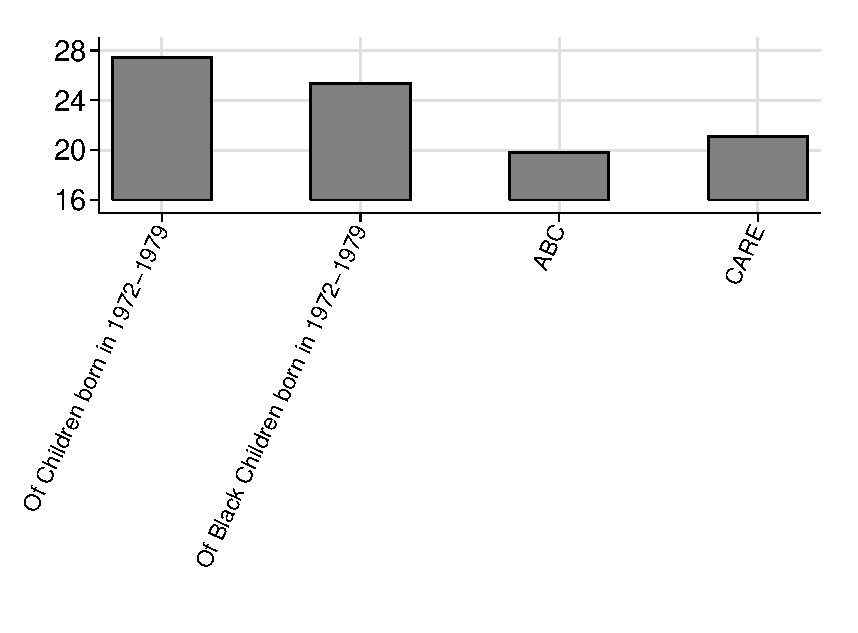
\includegraphics[height=2.3in]{output/abccarepsid_m_age0pool.eps}
\end{subfigure}%
\begin{subfigure}{.5\textwidth}
  \centering
  \subcaption{Average Maternal Years of Education} 
  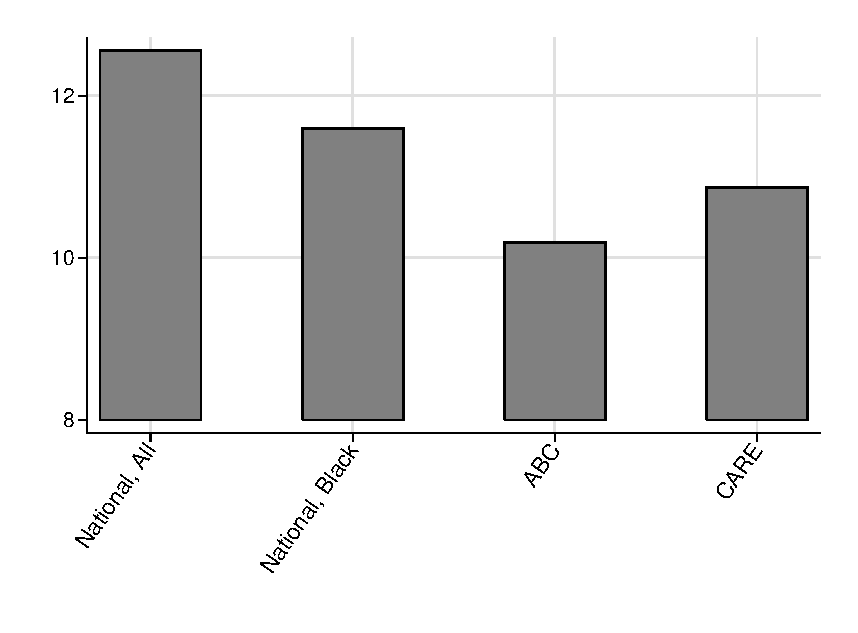
\includegraphics[height=2.3in]{output/abccarepsid_m_edu0pool.eps}
\end{subfigure}

\begin{subfigure}{.5\textwidth}
  \centering
  \subcaption{Proportion of Households with Father at Home}
  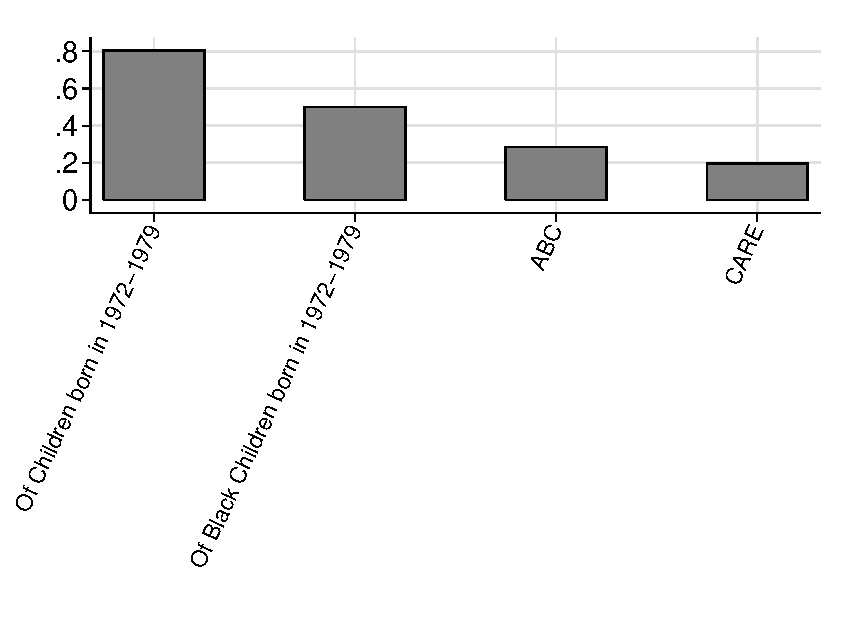
\includegraphics[height=2.3in]{output/abccarepsid_f_home0pool.eps}
\end{subfigure}%
\begin{subfigure}{.5\textwidth}
  \centering
  \subcaption{Median Parental Income in 1,000s of 2014 USD}
  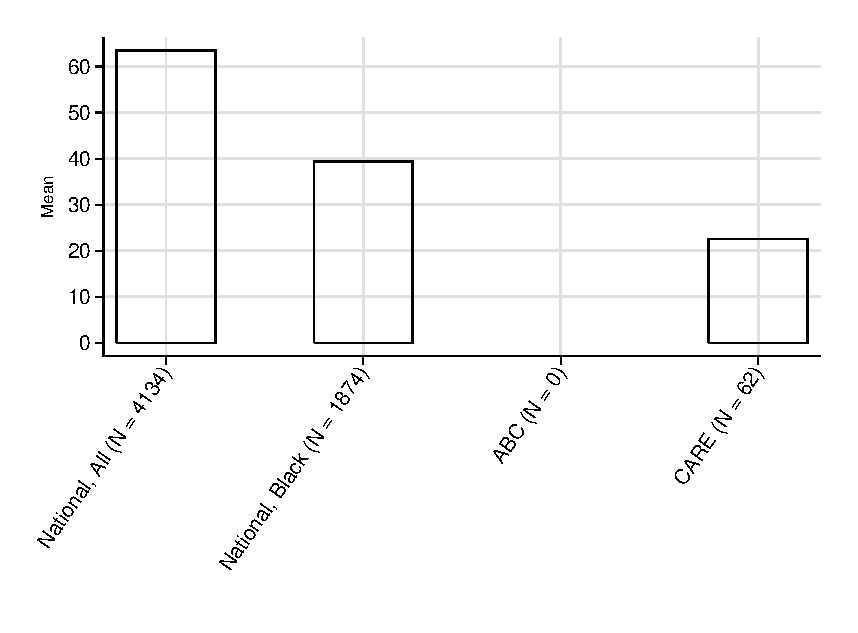
\includegraphics[height=2.3in]{output/abccarepsid_p_inc0pool.eps}
\end{subfigure}
\floatfoot{
\footnotesize
\noindent  Note: These panels plot four variable characteristics---mother's age, mother's education, an indicator of father at home, and parental income (in thousands of 2014 USD). In each panel, the first bar shows the national-level for a cohort born in the same years as the ABC and CARE individuals (1973-1979), obtained from the Panel Study of Income Dynamics (PSID). The second bar uses this same information restricted to black individuals. The third and fourth bars plot the same variables for ABC and CARE, pooling the treatment and control groups. We display the sample size for each calculation in parentheses next to the horizontal axis labels.
}
\end{figure}

\noindent To better understand the socio-economic status of the ABC participant families, we construct two comparison groups using the Panel Study of Income Dynamics (PSID), a nationally representative cohort of the children born in the same years as the ABC and CARE participants (1973-1979), and a similar cohort restricted to black children. We show a comparison in Figure~\ref{figure:baselineabccare}. Compared to both nationally representative groups, ABC children were, on average, significantly more disadvantaged; they were born in households with extremely low total parental income and to younger, less educated mothers, most of whom were raising their children without the support of a father. The CARE participants were similarly disadvantaged compared to nationally representative groups with respect to these basic household socio-demographic characteristics.\\

\subsection{Randomization Protocol and Compromises}

\subsubsection{ABC}

\noindent The first-phase randomization was paired at the family level, so pairs of siblings and twins were jointly randomized to either treatment or control.\footnote{Sibling pairs occurred when the two siblings were close enough in age such that both of them were eligible for the program.} Although we know that the pairing was based on HRI, maternal characteristics, number of siblings, and gender, we do not knows the original pairs. In total, 120 families took part in the study. As discussed below, our calculations indicate that 112 families participated in the initial randomization, while 8 families became part of the program as replacement for the families that withdrew.\\

\noindent There were some compromises to first-phase randomization. One control child participated in the program and three children in the treatment group did not participate due to the decisions of their families. We have information on these children and their families from birth until the end of elementary school. Four families moved out of the area before any data on them was collected and only data from adulthood is available. Two children in the control group were swapped into treatment at the request of local authorities, because they were considered to be at high-risk of developmental delay. Two additional children in the control group were dropped because they were diagnosed with a developmental delay, which made them ineligible for the program. Most of the data for these last four control children is available from birth until elementary school. Finally, four children died before age 5.\footnote{One child in the control group died at 3 months from cardiomyopathy and seizure disorder, and a second child in the control group died at 18 months from a cardiac arrest. One child in the treatment group died at 3 months from crib death, while the other died in a pedestrian accident at 50 months \citet{Ramey_Campbell_1984_AJMD}.} Thus, we classify 14 children as cases of attrition. Table~\ref{table:} compares their baseline characteristics with the baseline characteristics of the children who complied to the first-phase randomization.\\

\noindent \textbf{[JLG: Compliers vs. Attriters Table]}\\

\noindent The children who stopped participating in the program before they were 6 months old were replaced.\footnote{Three replacements are documented in \citet{Ramey_Campbell_1979_SR}. One is documented in correspondence with the program officers, which is available from the authors of this document upon request. The rest are implied by the number of children who participated of the randomization in each cohort.} Thus, the final first-phase sample consisted of 111 children (53 treatment children and 58 control children).\\

\noindent Prior to the second-phase randomization, 3 children in the control group of the first phase and 3 children in the treatment group of the first phase stopped being followed. One child in the control group and 8 children in the treatment group of the first phase did not participate in the second phase but later agreed to participate in the data collections during adulthood. This yielded a sample of 96 children, who were randomized to treatment (49) and control (47), independently of their status in the first phase. Three children in the control group did not comply with the randomization protocol by not participating, while all children in the control group adhered to their randomization status. Figure~\ref{fig:abc-flow} illustrates the randomization protocol for the two phases of the program.

\begin{center}
	\begin{figure}[H]
		\caption{Randomization Protocol and Treatment Compliance, ABC} \label{fig:abc-flow}
		\centering
		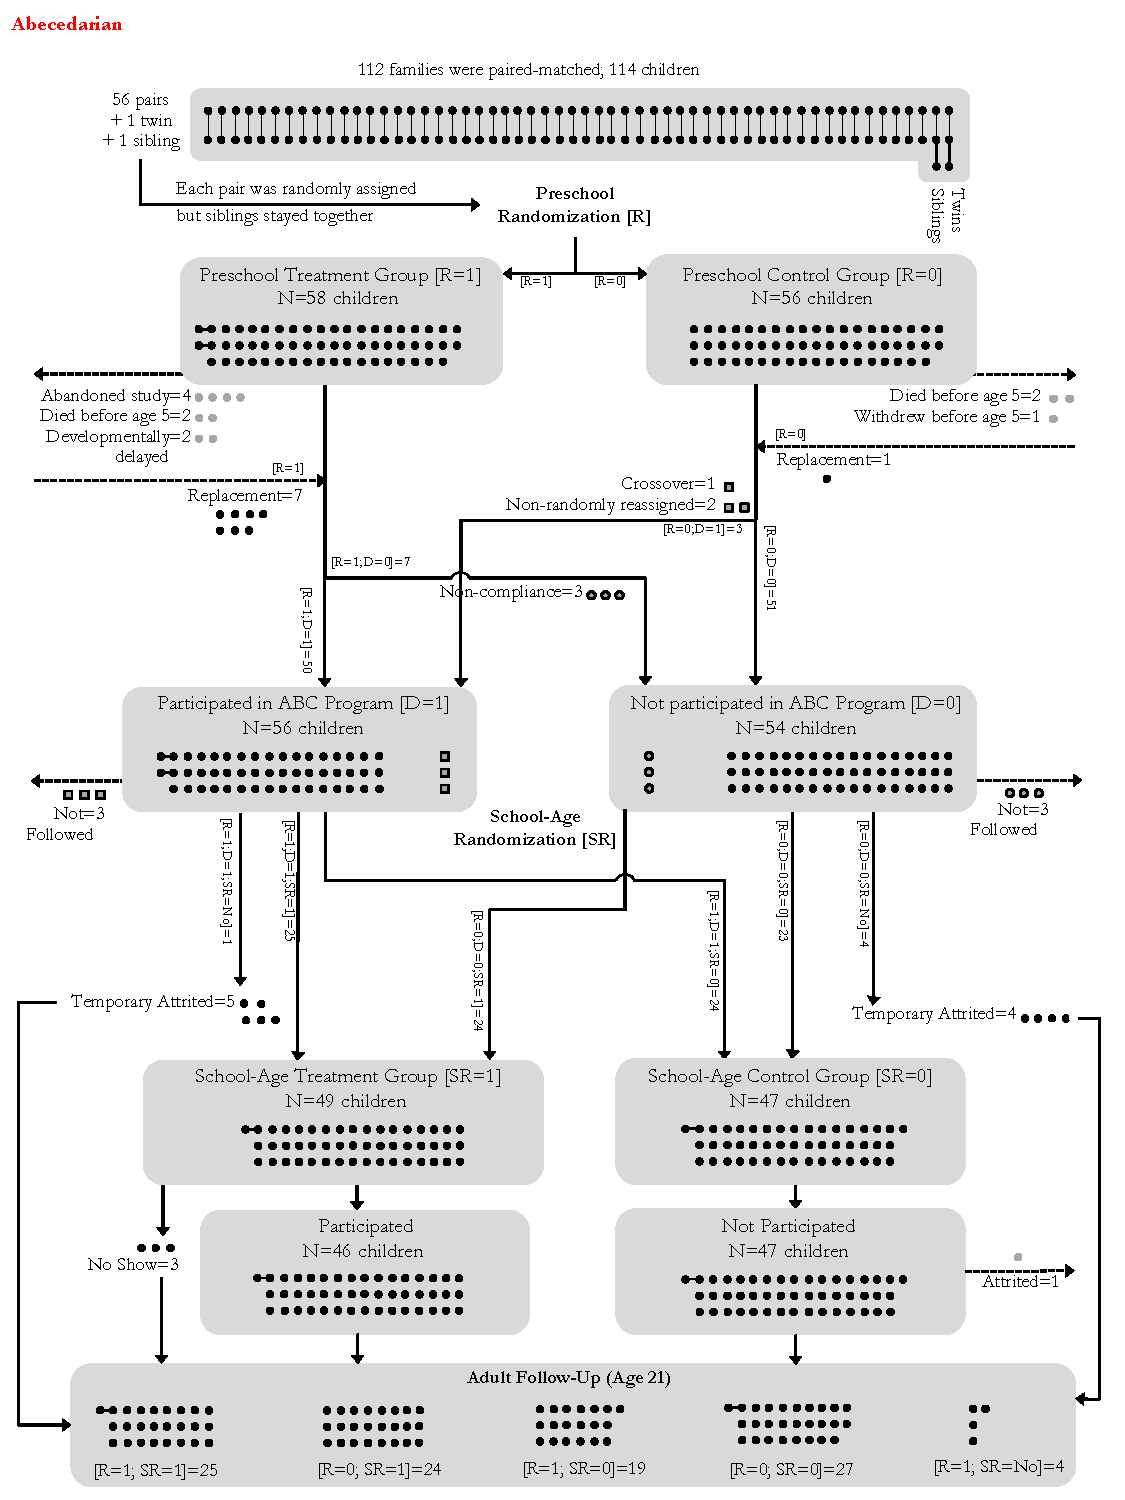
\includegraphics[width=.9\columnwidth]{output/abc_Diagram.pdf}
\floatfoot{
\footnotesize
\noindent
Sources: \cite{Ramey_Collier_etal_1976_CarolinaAbecedarianProject, Ramey_Smith_1977_AJMD,Ramey_Campbell_1979_SR,Ramey_Campbell_1984_AJMD}, internal documentation of the program, and own calculations. Note: The variable R represents randomization into treatment [R=1] or control [R=0] groups. After the original randomization, some children died or withdrew from the program early in life and were replaced. R also includes those replacements. Arrows pointing outside the diagram indicate children who left the study permanently. The variable P represents participation in the preschool-age program. The variable SR represents randomization into the school-age program [SR=1], or out of it [SR=0]. Some children were not randomized at school age [SR=No]. We use the term temporary attrited for children who did not participate in the study at school age, but were later interviewed in the age-21 followup.
}
	\end{figure}
\end{center}

\noindent While there was balance in observed, baseline characteristics between the children in the treatment and control groups in the two randomization phases (see Table~\ref{table:}), the explained compromises pose a methodological challenge that we assess when calculating the effects the program for all the outcomes and across all the ages for which we have data. We develop this further in Section~\ref{section:methodology}.\\

\noindent \textbf{[JLG: balance in observed characteristics for all both phases.]}\\

\subsubsection{CARE}

\noindent 
The randomization protocol in CARE was analogous to the first-phase randomization protocol in ABC. Importantly, it had no major compromises.\footnote{\citet{Bryant_et_al_1987_Carolina_Approach_TIECSE,Wasik_Ramey_etal_1990_CD,Burchinal_Campbell_etal_1997_CD}.} Of the 65 initial families, 23 were randomized to control, 25 to family education treatment, and 17 to family education and center-based childcare treatment. Two families in the family education treatment group had twins who were jointly randomized as in ABC. After randomization, the family of one child initially assigned to the family education and center-based childcare treatment refused its status and did not participate in the program. Within the first six months of treatment, one child assigned to this same group left the study due to family reallocation. Finally, one child who was assigned to the family education treatment group died. Figure~\ref{fig:care-flow} illustrates CARE's randomization and the flow of participants throughout the data follow-ups.\\

\begin{center}
	\begin{figure}[H]
		\caption{Follow-up Availability and Attrition, CARE} \label{fig:care-flow}
		\centering
		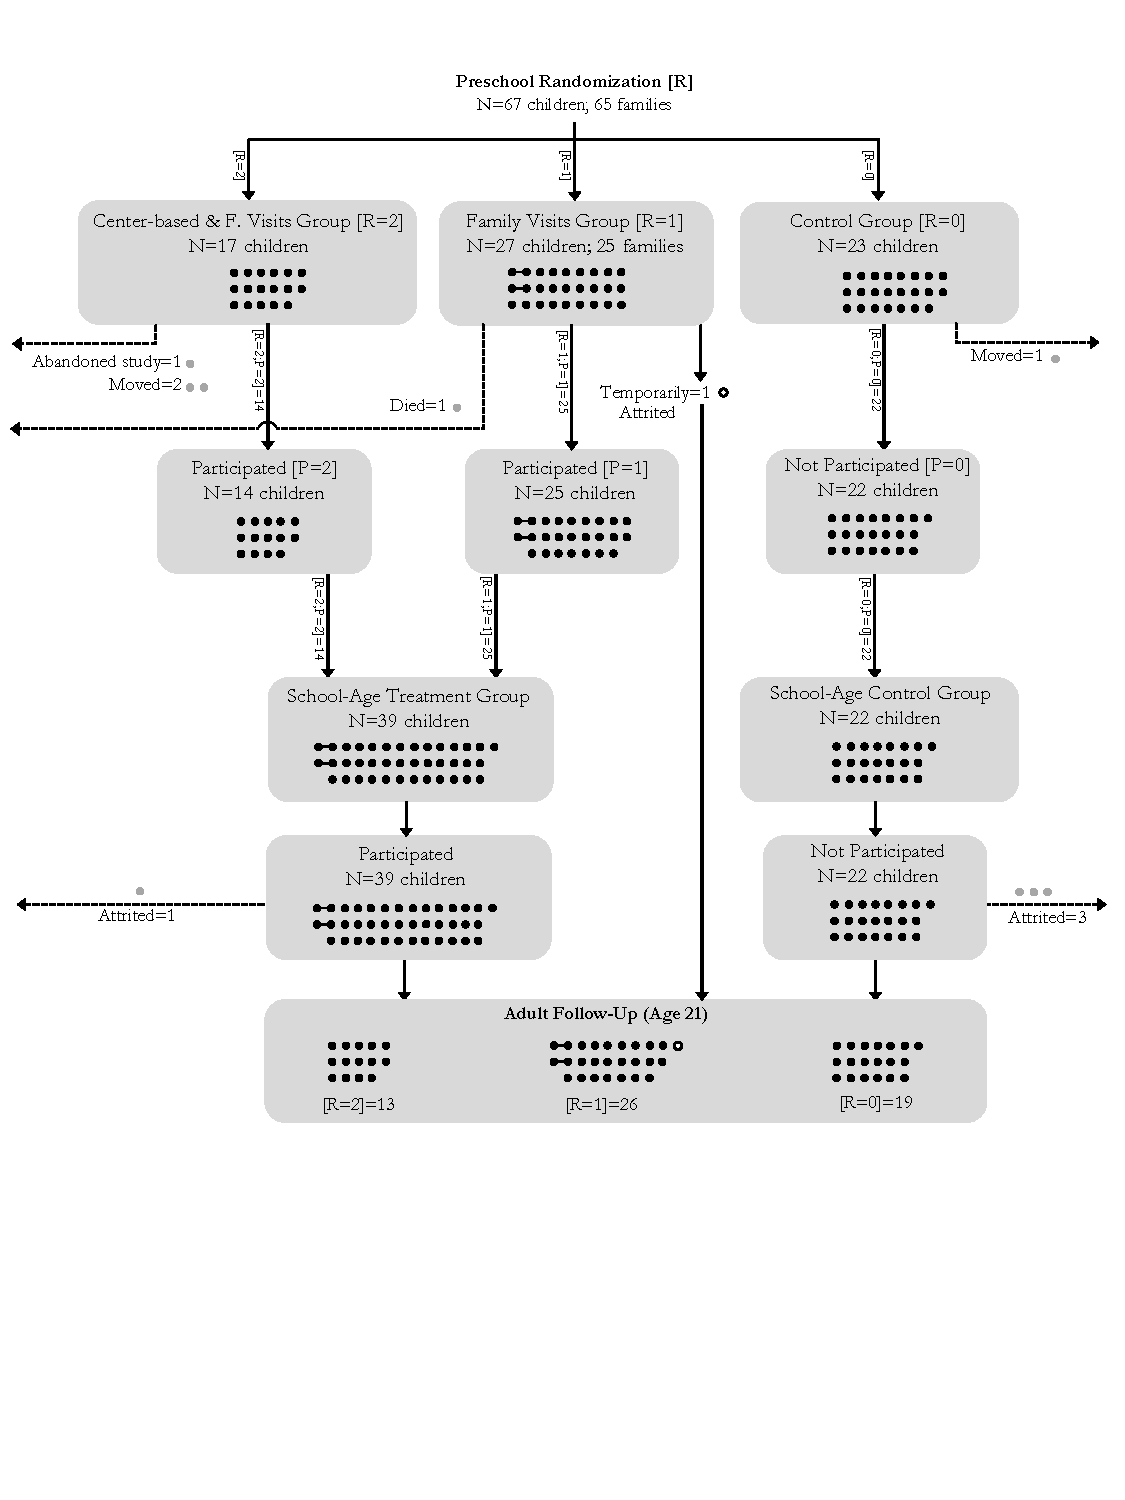
\includegraphics[width=.9\columnwidth]{output/care_Diagram.pdf}
\floatfoot{
\footnotesize
\noindent 
Sources: \cite{Wasik_Ramey_etal_1990_CD}, internal documentation of the program, and own calculations. Note: The variable R represents randomization into control [R=0], family education treatment [R=1], and family education and center-based childcare treatment [R=2]. Arrows pointing outside the diagram indicate children that left the study permanently. The variable P represents participation in the respective programs. Both the treatment groups continued into school-age with a home visitation program that was not randomized. We use the term temporarily attrited for children who did not participate in the study at school age, but were interviewed in the age-21 followup.}
	\end{figure}
\end{center}


\subsection{Treatment Substitution}

\noindent Clarifying the instances of treatment substitution is critical because it impacts the interpretation of simple comparisons between children in the control and the treatment groups, and poses a methodological challenge when answering policy-relevant questions.
In both programs, many children who did not have access to center-based childcare by random assignment were enrolled by their parents into alternative preschools. We document the take-up of alternative preschool here and propose a methodology to answer relevant policy-questions in Section~\ref{section:methodology}.\\

\begin{figure}[H]
		\caption{Treatment Substitution, ABC} \label{fig:treatsubabc}
		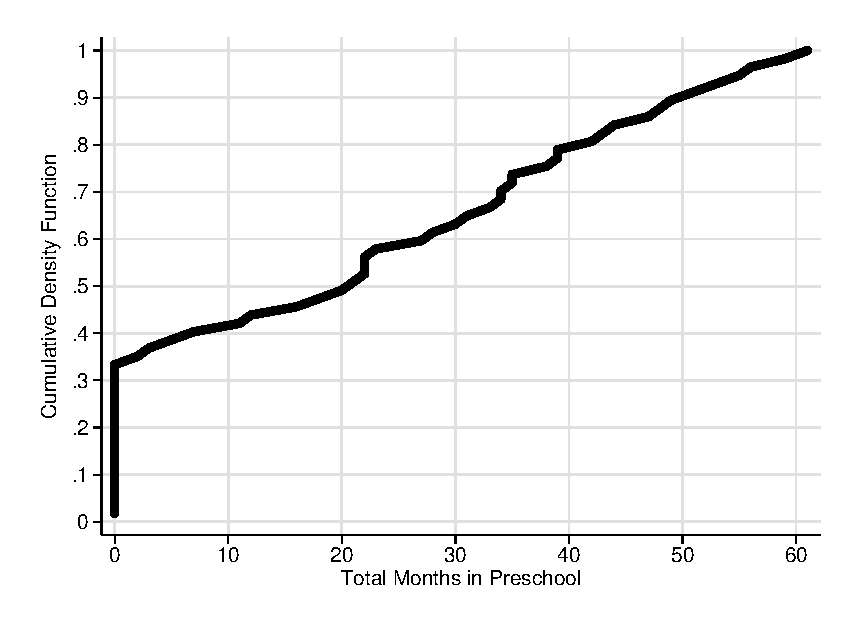
\includegraphics[width=.9\columnwidth]{output/abc_controlcontamination_months.eps}
\floatfoot{
\footnotesize
\noindent Note: This figure displays the cumulative density function of enrollment in alternative preschool for the control group in ABC.}
\end{figure}

\noindent In ABC, $70\%$ of control-group children enrolled in one of 11 local center-based childcare centers (see Figure~\ref{fig:treatsubabc}). All of these centers received federal subsidies and were therefore regulated by the Federal Interagency of Daycare Requirements. Their staff members were required to be trained in early childhood education and the centers were required to implement curricula designed to enhance cognitive, social, and linguistic competence in disadvantaged children.\footnote{\citet{Burchinal_etal_1989_CD_Daycare-Pre-K-Dev}.} In CARE, the control and family education treatment groups did not receive center-based childcare as part of the experimental design. However, slightly more than $70\%$ of the  former and $60\%$ of the latter were enrolled in alternative preschool by their parents, attending the same set of local center-based childcare centers as the ABC children in the control group (see Figure~\ref{fig:treatsubcare}).\\

\begin{figure}[H]
		\caption{Treatment Substitution, CARE} \label{fig:treatsubcare}
		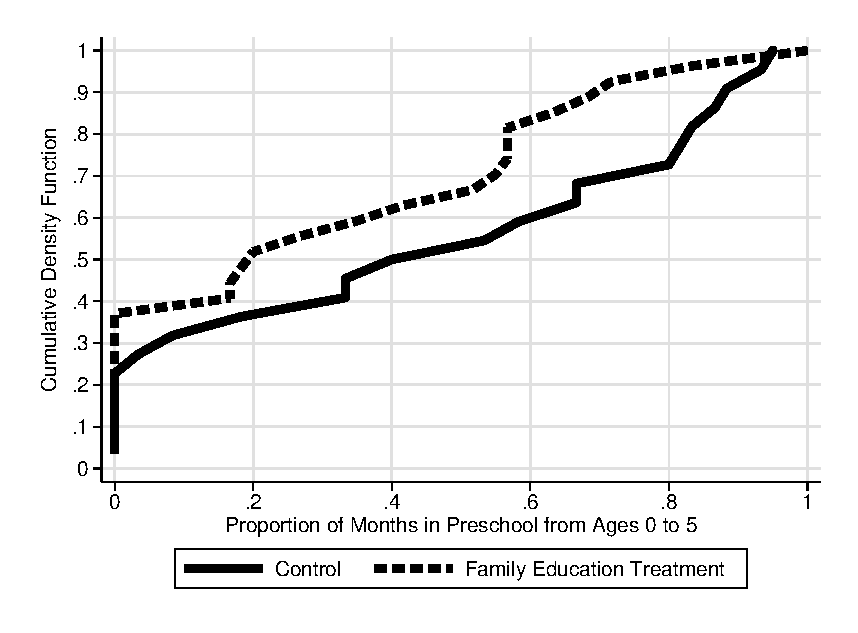
\includegraphics[width=.9\columnwidth]{output/care_controlcontamination_months.eps}
\floatfoot{
\footnotesize
\noindent Note: This figure displays the cumulative density function of enrollment in alternative preschool for the control and family education treatment groups in CARE.}
\end{figure}
 
\subsection{Program Description and Content}

\noindent The ABC and CARE programs shared many objectives and program components, as summarized in Table~\ref{tab:programcomparison}.\\

\begin{table}[H]
\begin{center}
\begin{threeparttable}
\caption{ABC and CARE, Programs Comparison} \label{tab:programcomparison}
\scriptsize
\scalebox{.9}{\begin{tabular}{L{4cm} L{7cm} L{5cm}}
\hline \hline
& \multicolumn{1}{c}{ABC}& \multicolumn{1}{c}{CARE}\\
\hline 
Program Overview &&\\
\hspace{.5cm} Years Implemented &1972--1982&1978--1985\\
\hspace{.5cm} Age of Entry/Exit & birth to 5 years old &\checkmark\\
\hspace{.5cm} Initial Sample &122&64\\
\hspace{.5cm} \# of Cohorts &4&2\\
\midrule
Eligibility & socio-economic disadvantage according to a multi-factor index (see Section \ref{section:eligibility})&\checkmark\\
 \midrule
Control &&\\
\hspace{.5cm} N &54&23\\
\hspace{.5cm} Compensation & Diapers from birth to age 3, unlimited formula from birth to 15 months & \checkmark \\
\hspace{.5cm} Treatment Substitution & 70\% & $\sim$ 70\%\\
\midrule
Treatment & Center-based childcare & Center-based childcare and family education\\
\hspace{.5cm} \textbf{Center-base} &&\\
\hspace{.5cm} \textbf{Childcare} &&\\
\hspace{.5cm} N &57&17\\
\hspace{.5cm} Intensity &6.5--9.75 hours a day for 50 weeks per year&\checkmark\\
\hspace{.5cm} Components & Instruction, medical care, nutrition, social services &\checkmark\\
\hspace{.5cm} Staff-to-child Ratio &1:3 during ages 0--1 &\checkmark\\
&1:4--5 during age 1--4 &\checkmark\\&1:5--6 during ages 4--5 &\checkmark\\
\hspace{.5cm} Staff Qualifications &Mixed diplomas; experienced&\checkmark\\
\hspace{.5cm} \textbf{Family Education} & Not part of the program &24\\
\hspace{.5cm} Intensity && One hour-long home visits. 2--3 per month during ages 0--3. 1--2 per month during ages 4--5\\
\hspace{.5cm} Curriculum & & Social and mental stimulation; parent-child interaction\\
\hspace{.5cm} Staff-to-child Ratio &&1:1\\
\hspace{.5cm} Staff Qualifications &&Home visitor training\\
\midrule
 School-age Treatment \\
 \hspace{.5cm} N&46&39\\
\hspace{.5cm} Intensity &Every other week& \checkmark\\
\hspace{.5cm} Components &Parent-teacher meetings& \checkmark\\
\hspace{.5cm} Curriculum & Reading and math &\checkmark\\
\hspace{.5cm} Staff-to-child Ratio &1:1&\checkmark\\
\hspace{.5cm} Staff Qualifications &Graduate degree and training in special education & \checkmark\\
\midrule
Data Availability \\
Questionnaires & Ages 0--5, 8, 12, 15, 21, 30--34 & Ages 0--5, 8, 12, 21, 30--34 \\
Parent Interview & Ages 0--5, 8, 12, 15, 21& Ages 0--5, 9, 12 \\  
Health Follow-up & Ages 30--34&\checkmark\\
\hline \hline
\end{tabular}}
\footnotesize
\begin{tablenotes}
\item Note: This table compares the main elements of ABC and CARE, summarized within this section.
\end{tablenotes}
\end{threeparttable}
\end{center}
\end{table}

\noindent ABC and CARE had a common principle objective: prevent mental retardation by enhancing development from birth and foster school readiness for disadvantaged children.\footnote{Note that the clinical understanding of mental retardation was once associated with disadvantages that hindered early-life development \citep{Mental-Retardation_America_2004_BOOK_NYU}.} The different curricula implemented through center-based childcare across programs and cohorts had the following common goals: (i) support language and cognitive development; (ii) develop socio-emotional competencies that were considered to enable school readiness---e.g. task orientation, emotional self-expression, independence, sharing, and cooperation.\footnote{\citet{Sparling_1974_Synth_Edu_Infant_SPEECH,Ramey_Collier_etal_1976_CarolinaAbecedarianProject,Ramey-etal_2012-ABC}.} The curricula evolved each year based on studies of children's data completed by the programs' staff.\footnote{\citet{Ramey-etal_1975_AJoMD,Finkelstein_1982_Day_Care_YC,Haskins_1985_CD}.}$^{,}$\footnote{The curricula implemented in the first phases of ABC and CARE, including Tools of Mind, shared an emphasis on self regulation---e.g., goal setting and self-reflection--- and opportunities for language development. Language development, including phonics and reading skills, is also an important element in other widely implemented curricula such as Opening the World of Learning.}$^{,}$\footnote{Two other renowned early childhood education programs are worth comparing to ABC and CARE. The Infant Health and Development Project (IHDP) was based on the first phase of CARE. IHDP had a single treatment group, which was very similar to the center-based childcare and family education treatment group of CARE. The curricula implemented both at home and at center-based childcare were very similar. The main difference is that the first phase of CARE lasted 5 years, while IHDP lasted 3 years and did not have a second phase. Both ABC and CARE were notably different from the Nurse Family Partnership (NFP) program. NFP had fewer visits and began in the pre-natal period. Mothers received monthly visits during pregnancy and one visit every two months from when the child was born until the age of 2. The visitors were nurses and they tried to help women build relationships with friends and family to create a support network for their children. A common element of the three programs is that the visitors helped parents use community resources when solving their everyday problems.}\\

\noindent Both treatment groups in CARE had home visits, with the main objectives of helping parents think about everyday problems that could adversely affect the relationship they have with their children and brainstorm solutions, as well as improving the general skills necessary for parenting. Usually, the home visits were weekly and one hour long. Between birth and the age of 3, the participants in the family education and center-based childcare and family education groups received, on average, 2.5 and 2.7  visits a month respectively. At ages 4 and 5, the average frequency decreased to 1.4 and 1.1 visits per month, respectively.\\ 

\noindent The first phases of ABC and CARE were conducted in conjunction with a longitudinal medical research study on infectious respiratory diseases in group environments.\footnote{\citet{Henderson-et-al_1982_NEJoM}.} This allowed the children to have comprehensive medical care in the same center in which they received center-based childcare. The children who attended the center received daily screenings to detect any signs of illness. This included all the children in the treatment group of ABC and all the children in the center-based childcare and family education group of CARE. The first cohort of the control group of ABC also received frequent medical check-ups during the first year of the first-phase of the program.\\

\noindent The children assigned to treatment in the first phase of ABC also received primary pediatric care by a family nurse practitioner and a licensed practical nurse, who were supervised by a pediatrician who was on continuous duty at the center-based childcare center. This care consisted of wellness check-ups, immunizations, parental counseling, and initial assessments of illnesses. Like the other treatment components, pediatric care was free of charge. Unfortunately, there is no documentation or corresponding evidence of whether this part of treatment was available for either of the treatment groups of CARE.\\

\noindent All participants center-based childcare in both programs were provided breakfast, lunch, and an afternoon snack, planned by a nutritionist. Children in the control groups of both programs received diapers from birth until the age of 3, and an unlimited supply of bottled formula from birth until 15 months. None of the control groups of  ABC or CARE or the family education treatment group of CARE received any medical care, with the exception of the first cohort of the control children in ABC, as explained above.\\

\noindent The children in ABC were subject to a second randomization protocol, when they were assigned to either treatment or control independently of their status in the first-phase. The children in CARE were not subject to a second randomization protocol. Instead, both the family education and the center-based childcare and family education treatment groups were given second-phase treatment. The control group of the first phase continued to be the control group of the second stage. The second-phase, also referred to as school-age treatment, lasted for the first three year of elementary school and consisted of home visits by a teacher. The objective of the visits was to increase exposure to reading and mathematics and promote parental involvement in the learning process. The visits happened every two weeks in the presence of the parents. The teachers discussed the children's programs with the parents and helped parents with issues related to literacy, housing, and medical care.\\ 

\subsection{Data} \label{section:data}

\noindent The data availability from both ABC and CARE is summarized in Table~\ref{tab:ecvars_1}. The collection processes in both programs were analogous by design. The treatment and control groups were followed into adulthood with relatively low attrition. For ABC, children were followed-up with annually through elementary school and and at ages 12, 15, 21, and 30. Health and administrative crime data were collected when the children reached their mid-30s. For CARE, the exact same follow-ups are available with the exception of the one at age 15.\\

\begin{sidewaystable}[H]
\small
\caption{Early Childhood Data (Part I)}
\label{tab:ecvars_1}
\centering
\begin{adjustbox}{max width=\textwidth, max height=\textheight,keepaspectratio}
\begin{threeparttable}
\tiny
\begin{tabular}{L{3cm} C{3.5cm} C{4cm} C{1.5cm} C{1.5cm}  C{6cm}}
\toprule
\textbf{Category}	&	\textbf{Sub-Category}	&	\textbf{Description}	&	\textbf{ABC Age}  	&  \textbf{CARE Age}  & 	\textbf{Measure}	\\ \midrule
Demographics	&	Gender	&	Gender of child	&	Birth, 18, 30, 42, 54	&	 Birth, 18, 30, 42, 54	&	Demographic Interview	\\
	&	\\
	&	Race	&	Race/Cultural identity of child	&	Birth, 18, 30, 42, 54	&	 Birth, 18, 30, 42, 54	&	 Demographic Interview\\
	&	\\
	&	Birth Date	&	Date of birth of child	&	Birth, 18, 30, 42, 54	& 	Birth, 18, 30, 42, 54	&	 Demographic Interview	\\ \midrule
Cognitive Assessments	&	Language Ability	&	Auditory association, Verbal expression, etc. 	&	36, 42, 48, 54	&	30, 42, 54	&	ITPA$^{ABC}$, GPB$^{ABC}$, PLP$^{ABC}$, MSCD \\
	&	\\
	&	Intelligence Levels	&	SBIS 	&	24, 36, 48, 60	&	24, 36, 48, 60	&	SBIS	\\
	&		&	WPPSI	&	60	&	60	&	WPPSI	\\
	&		&	BSID 	&	3, 6, 9, 12, 18, 24	&	6, 12, 18, 24		&	BSID	\\
	&		&	UOSPD	&	15	&	- 	&	UOSPD$^{ABC}$	\\
	&		&	RPM	&	60	&	-	&	RPM$^{ABC}$	\\
	&	\\
	&	Quantitative	 &	BSID 	&	3, 6, 9, 12, 18, 24	&	6, 12, 18, 24		&	BSID	\\
	&		&	MSCD 	&	30, 42, 54		&	30, 42, 54	&	MSCD	\\
	&	\\
	&	Memory	&	BSID 	&	3, 6, 9, 12, 18, 24	& 	6, 12, 18, 24		&	BSID	\\
	&		&	MSCD 	&	30, 42, 54	&	30, 42, 54	&	MSCD	\\
	&	\\
	&	Motor Development	&	BSID 	&	3, 6, 9, 12, 18, 24	&	6, 12, 18, 24		&	BSID\\
	&		&	MSCD 	&	30, 42, 54	&	30, 42, 54	&	MSCD	\\
	& 	\\
	&	Critical Thinking	&	Curiosity	&	30, 36, 42, 48, 54, 60, 66, 72	& - &	Infant Behavior Inventory$^{ABC}$	\\ \midrule
Non-Cognitive Assessments	&	Social Skills	&	Positive social response	&	30, 36, 42, 48, 54, 60, 66, 72	&	6, 12, 18, 24		&	Infant Behavior Inventory$^{ABC}$, Bayley Infant Inventory$^{CARE}$	\\
	&		&	Creativity	&	30, 36, 42, 48, 54, 60, 66, 72	&	- 	&	Infant Behavior Inventory$^{ABC}$	\\
	&	\\
	&	Self-Control	&	Locus of control	&	3, 18	&	6, 18	& 	RIES	\\
	&		&	Distractibility, Attentiveness	&	30, 36, 42, 48, 54, 60, 66, 72	&	6, 12, 18, 24		&	Infant Behavior Inventory$^{ABC}$, Bayley Infant Inventory$^{CARE}$	\\
	&	\\
	&	Emotional Health	&	KRT	&	24, 36, 48, 60	&	24, 30, 36, 42, 48, 60	&	KRT	\\
	&	\\
	&	Self-Consciousness	&	Self-consciousness	&	30, 36, 42, 48, 54, 60, 66, 72	&	-	&	Infant Behavior Inventory$^{ABC}$	\\
\bottomrule
\end{tabular}
\begin{tablenotes}
\scriptsize
\item Sources: Authors' description. \\	
\item Note: This table describes the major categories of variables that were measured for ABC and CARE subjects up to age 6. ABC and CARE ages are measured in months. This is not an exhaustive list of variables, nor does it include variables from auxiliary data. Instruments or questionnaires available for only one of the studies are indicated with the superscript $^{ABC}$ or $^{CARE}$.  \textbf{Abbreviations are as follows.} ITPA: Illinois Test of Psycholinguistic Ability. GPB: Gordon Psycholinguistic Battery. PLP: Preschool Language Performance. MSCD: McCarthy Scales of Children's Development. BSID: Bayley Scales of Infant Development and Infant Behavior. UOSPD: Uzgiris-Hunt Ordinal Scales of Psychological Development. RPM: Raven's Progressive Matrices. RIES: Rotter's Internality-Externality Scale. KRT: Kohn and Rosman Test Behavior Inventory.
\end{tablenotes}
\end{threeparttable}
\end{adjustbox}
\end{sidewaystable}




\begin{sidewaystable}[H]
\small
\caption{Early Childhood Data (Part II)}
\label{tab:ecvars_2}
\centering
\begin{adjustbox}{max width=\textwidth, max height=\textheight,keepaspectratio}
\begin{threeparttable}
\tiny
\begin{tabular}{L{3cm} C{3.5cm} C{4cm} C{1.5cm} C{1.5cm}  C{6cm}}
\toprule
\textbf{Category}	&	\textbf{Sub-Category}	&	\textbf{Description}	&	\textbf{ABC Age}  	&  \textbf{CARE Age}  & 	\textbf{Measure}	\\ \midrule
Family Environment	&	Family Members	&	Number of primary caretakers	&	Birth, 18, 30, 42, 54	&	18, 30, 42, 54, 60	&	Demographic Interview	\\
	&		&	Relationship with family members, including father, mother, siblings, etc.	&	Birth, 18, 30, 42, 54	&	18, 30, 42, 54, 60	&	Demographic Interview	\\
	&		&	Number of siblings	&	Birth, 18, 30, 42, 54	&	Birth, 18, 30, 42, 54, 60	&	Demographic Interview	\\
	&		&	Marital status of parents	&	Birth, 18, 30, 42, 54	&	Birth, 18, 30, 42, 54, 60	&	Demographic Interview	\\
	&		&	Marital conflicts between parents	&	6, 18	&	Birth, 6, 18, 36	&	Demographic Interview$^{CARE}$, Parental Attitudes Research Inventory	\\
	&		& Father at home & 18, 30, 42, 54  & 18, 30, 42, 54, 60 & Demographic Interview \\
	&	\\
	&	Family Economic Environment	&	Parents' occupation	&	Birth, 18, 30, 42, 54	& 	Birth, 18, 30, 42, 54, 60		&	Demographic Interview	\\
	&								& Mother works & 18, 30, 42, 54 & 18, 30, 42, 54, 60 & Demographic Interview \\
	&		&	Source of child support	&	Birth, 18, 30, 42, 54	&	18, 30, 42, 54, 60	&	Demographic Interview	\\
	&		&	Family income	&	Birth, 18, 30, 42, 54	&	Birth, 18, 30, 42, 54, 60	&	Demographic Interview	\\
	&	\\
	&	Parents and Home Environment & Parents' authority, warmth, family conflict, etc. & 6, 18, 30, 42, 54 & 6, 12, 18, 30, 42, 54 & Parent Interview \\
	&	\\
	&	Family Social Status	&	Parents' education background	&	Birth, 18, 30, 42, 54	&	Birth, 18, 30, 42, 54, 60		&	Demographic Interview	\\
	&		&	Risk taking of family members	&	Birth	&	- 	&	Parent Interview$^{ABC}$	\\
	&	\\
	&	Family Members' Physical Health	&	Health issues of parents	&	Birth	&	Birth	&	Parent Interview	\\
	&		&	Pregnancy history	&	Birth	&	Birth	&	Parent Interview	\\ \midrule
Childcare	&	Day-care Experience	&	Time and location of day-care, Age when begin	&	Birth, 18, 30, 42, 54	&	18, 30, 42, 54	&	Demographic Interview	\\
			&						& 	Home visits &	-	&	6, 18, 30, 42, 54, 60	& Home Visit Data$^{CARE}$ \\
	&	\\
	&	Parental Care	&	Maternal warmth, Maternal involvement with child	&	6, 18, 30, 42, 54	&	6, 12, 18, 30, 42, 54	&	Home Stimulation	\\
	&		&	Provision of appropriate play materials	&	6, 18, 30, 42, 54	&	 6, 12, 18, 30, 42, 54	&	Home Stimulation	\\
	&		&	Avoidance of restriction and punishment	&	6, 18, 30, 42, 54	&	6, 12, 18, 30		&	Home Stimulation	\\
	&		&	Authoritarian control	&	6, 18, 30, 42, 54	&	6, 12, 18, 30, 36, 42, 102		&	Home Stimulation, Parental Attitudes Research Inventory	\\
	&		&	Democratic attitudes	&	6, 18	&	6, 18, 36	&	Parental Attitudes Research Inventory	\\
	&		&	Hostility and rejection	&	6, 18	&	6, 18, 36	&	Parental Attitudes Research Inventory	\\
	&		&	Parents' knowledge of childcare	&	Birth	&	-	&	Parent Interview$^{ABC}$	\\ \midrule
Physical Health	&	Growth Data	&	Height, Weight, Head circumference, etc.	&	3, 6, 9, 12, 18, 24, 36, 48, 60	&	Birth, 6, 12, 18, 24, 36, 48, 60	&	Growth Measures	\\
\bottomrule
\end{tabular}
\begin{tablenotes}
\scriptsize
\item Sources: Authors' description. \\	
\item Note: This table describes the major categories of variables that were measured for ABC and CARE subjects up to age 6. ABC and CARE ages are measured in months. This is not an exhaustive list of variables, nor does it include variables from auxiliary data.  Instruments or questionnaires available for only one of the studies are indicated with the superscript $^{ABC}$ or $^{CARE}$.
\end{tablenotes}
\end{threeparttable}
\end{adjustbox}
\end{sidewaystable}



\begin{sidewaystable}[H]
\begin{threeparttable}
\small
\caption{Childhood and Adolescence Data (Part I)} \label{tab:youthvars_1}
\centering
\tiny	
\begin{tabular}{L{3.5cm} C{3.5cm} C{5cm} C{1.5cm} C{1.5cm} C{6cm}}
\toprule
\textbf{Category}	&	\textbf{Sub-Category}	&	\textbf{Description}	&	\textbf{ABC Age}  	&  \textbf{CARE Age}  & 	\textbf{Measure}	\\ \midrule
Cognitive Assessment	&	Language Ability	&	Adaptive Language Inventory	&	6, 7, 8	&	6, 7, 8	&	Adaptive Language Inventory	\\
	&		&	Language Questionnaire	&	12	&	- 	&	Language Questionnaire$^{ABC}$	\\
	&		&	MSCD 	&	7	&	- 	&	MSCD$^{ABC}$	\\
	&	\\
	&	Intelligence Tests	&	SBIS	 &	6	&	7	&	SBIS	\\
	&		&	 WIS	&	6, 7, 8, 12, 15	&	6, 8	&	WIS	\\
	&		& Kaufman$^{CARE}$ & 	-	& 6 & Kaufman$^{CARE}$ \\
	&	\\
	&	Quantitative Skills	&	MSCD$^{ABC}$ 	&	7	&	-	&	MSCD$^{ABC}$ 	\\
	&	\\
	&	Memory	&	MSCD$^{ABC}$ 	&	7	&	-	&	MSCD$^{ABC}$	\\
	&	\\
	&	Motor Skills	&	MSCD$^{ABC}$ 	&	7	&	-	&	MSCD$^{ABC}$	\\ \midrule
Non-Cognitive Assessment	&	Interpersonal Skills	&	Gets along with people	&	6, 8, 12, 15	& 	8, 12	&	PEI, CAS, PMI$^{ABC}$, SAI$^{ABC}$, Subject Interview$^{ABC}$, Quality Rank$^{CARE}$	\\
	&		&	Relationship with the other sex	&	15	&	- 	&	 SAI$^{ABC}$, Subject What I Am Like (Harter)$^{ABC}$	\\
	&	\\
	&	Critical Thinking	&	Thinks for self, questions things	&	6, 8	 &	8, 12	&	PEI, Harter Child$^{CARE}$, CBI	\\
	&		&	Concept Attainment Kit	&	6, 7, 8	&	- 	&	Concept Attainment Kit$^{ABC}$	\\
	&	\\
	&	Self-Control	&	Distracted in class	&	6, 7, 8, 12, 15	&	12	&	SCAN$^{ABC}$, CBI, WPB$^{ABC}$, PMI$^{ABC}$, SAI$^{ABC}$, Self-Evaluation Inventory$^{ABC}$	\\
	&		&	Locus of control	&	15	&	- 	&	Nowicki-Strickland Data, Pearlin Mastery Scale$^{ABC}$	\\
	&	\\
	&	Work Ethic	&	Task Orientation	&	6, 7, 8, 12, 15	&	6, 7, 8, 9, 12 	&	SCAN$^{ABC}$, CBI, PMI$^{ABC}$		\\
	&	\\
	&	Emotional Health	&	Harms self, suicidal thoughts	&	8, 12, 15	&	8, 12	 	&	Achenbach Parent,  Subject Risk Taking Survey$^{ABC}$		\\
	&		&	Depression, anxiety, fear, etc.	&	6, 7, 8, 12, 15	&	7, 8, 9, 12	&	KRT, CAS, ETS,  Achenbach Parent	\\
	&	\\
	&	Social Activities	&	Athletic activities	&	8, 12, 15	&	8, 12		&	Achenbach Parent, SAI$^{ABC}$, Subject What I Am Like (Harter)$^{ABC}$, PEI$^{CARE}$	\\
	&		&	Participant of organizations, e.g. religions	&	8, 12, 15	&	8, 12	&	Achenbach Parent, SAI$^{ABC}$, Subject Interview$^{ABC}$	\\
	&		&	Reading list	&	12, 15	&	12	&	CAS, SAI$^{ABC}$	 \\
	&		&	TV/music	&	12, 15	&	12	&	CAS, SAI$^{ABC}$	, Television Checklist$^{ABC}$		\\
	&	\\
	&	Self-Consciousness	&	Self-conscious emotions	&	8, 12, 15	&	8, 12	&	Achenbach Parent, Subject What I Am Like (Harter)	\\ \bottomrule
	\end{tabular}
\begin{tablenotes}
\scriptsize
\item Sources: Authors' descriptions. \\
\item Note: This table describes the major categories of variables that were measured for ABC and CARE subjects at ages 6 to 18. ABC and CARE age are measured in years. This is not an exhaustive list of variables, nor does it include variables from auxiliary data.  Instruments or questionnaires available for only one of the studies are indicated with the superscript $^{ABC}$ or $^{CARE}$. \textbf{Abbreviations are as follows.}  MSCD: McCarthy Scales of Children's Development. SBIS: Stanford-Binet Intelligence Scale. WIS: Wechsler Intelligence Scale for Children. KRT: Kohn and Rosman Test Behavior Inventory. WJCA: Woodcock-Johnson Test of Cognitive Abilities. PEI: Parents as Educator Interview. CAS: Child Assessment Schedule. PMI: Psychosocial Maturity Inventory. SAI: Social Adjustment Inventory for Children and Adolescents. SCAN: Schedule of Classroom Activity Norms. CBI: Classroom Behavior Inventory. WPB: Walker Problem Behavior Checklist. ETS: Emotional/Activity/Sociability/Impulsivity Temperament Survey. FES: Family Environment Scale. PIAT: Peabody Individual Achievement Test. CAT: California Achievement Test. MARS: Mid-Adolescence Rating Scale Data.
\end{tablenotes}
\end{threeparttable}
\end{sidewaystable}

	
	
\begin{sidewaystable}[H]
\begin{threeparttable}
\small
\caption{Childhood and Adolescence Data (Part II)} \label{tab:youthvars_2}
\centering
\tiny
\begin{tabular}{L{3.5cm} C{3.5cm} C{5cm} C{1.5cm} C{1.5cm} C{6cm}}
\toprule
\textbf{Category}	&	\textbf{Sub-Category}	&	\textbf{Description}	&	\textbf{ABC Age}  	&  \textbf{CARE Age}  & 	\textbf{Measure}	\\ \midrule
Family Environment	&	Family Members	&	Number of adults in house	&	6, 8, 12, 15	&	8, 12	&	PEI, Parent Interview, Subject Person In Household$^{ABC}$		\\
	&		&	Relationship with family members, including father, mother, siblings, etc.	&	6, 8, 12, 15	&	8, 12	&	PEI, FES, SAI, Subject Interview$^{ABC}$, Adult Self Report$^{ABC}$, Parent Interview, Achenbach Parent	\\
	&		&	Number of siblings	&	6, 8, 12, 15	&	7, 8, 12	&	PEI$^{ABC}$, Parent Interview	\\
	&		&	Marital status of parents	&	6, 8, 12, 15	&	7, 8, 12	&	PEI$^{ABC}$	, Parent Interview	\\
		&		& Father at home & 18, 30, 42, 54  & 18, 30, 42, 54, 60 & Demographic Interview \\
	&	\\
	&	Parents' Education Style	&	Role of parents in education	&	6, 8	&	8, 12	&	PEI, Parent Interveiw$^{CARE}$	\\
	&		&	Parents' education beliefs \& methods&	6, 8	&	8, 12 	&	PEI, Parent Interview$^{CARE}$		\\
	&		&	Parents' aspiration \& attitudes towards child	&	6, 8, 12, 15	&	8, 12	&	PEI, Parent Interview	\\
	&	\\
	&	Family Economic Environment	&	Parents' occupation	&	6, 8, 12, 15	&	7, 8, 12	&	PEI$^{ABC}$, Parent Interview	\\
		&							& Mother works & 9 & 5, 7, 8 & Demographic Interview \\
	&		&	Source of child support	&	6, 8, 12, 15	&	7, 8, 12	&	PEI$^{ABC}$, Parent Interview	\\
	&		&	Family income	&	6, 8, 12, 15	&	7, 8, 12	&	PEI$^{ABC}$, Parent Interview	\\
	&	\\
		&	Parents and Home Environment & Parents' authority, warmth, family conflict, etc. & 8 & 8 & Parent Interview \\
	&	\\
	&	Family Social Status	&	Parents' education background	&	6, 8, 12, 15	&	7, 8, 12	&	PEI$^{ABC}$, Parent Interview	\\
	&		&	Criminal history and risk taking of family members	&	8, 12, 15	&	- 	&	Subject Taylor Life Events$^{ABC}$, Parent Interview$^{ABC}$	\\
	&	\\
	&	Family Members' Physical Health	&	Health issues of adults in house	&	8, 12, 15	&	12	&	Parent Interview, Subject Taylor Life Events$^{ABC}$	\\ 	\midrule
Academic Achievements	&	Standardized Tests	&	Reading, mathematics, and language abilities	&	6, 7, 8, 12	&	6, 8, 9,12	&	CAT$^{ABC}$, PIAT$^{ABC}$, WJCA	\\
		&	\\
	&	Performance in Schoolwork	&	Drop in grades	&	12, 15		&	12	&	CAS	\\
	&		&	Lack of interest in school	&	12, 15		&	12	&	CAS	\\
	&		&  Total years in special education & 17 & 11 & Retention and Special Services Data \\
	&		&  Total years retained in school & 17 & 11 & Retention and Special Services Data \\  \midrule
Physical Health	&	Health Issues	&	Health issues of subject	&	8, 12, 15	&	8, 12	&	Achenbach Parent, Subject Interview$^{ABC}$, Adult Self Report$^{ABC}$, PEI$^{CARE}$, Parent Interview$^{CARE}$	\\
	&	\\
	&	Growth	&	Vision, weight, height	&	8	&	8	&	Growth Data	\\
	&	\\
	&	Teenage Pregnancy	&	Teenage Pregnancy	&	15	&	- 	& Subject Interview$^{ABC}$		\\ \midrule
Social Conduct	&	Law Breaking	&	Felony, Time spent incarcerated	&	15	&	- 	&	MARS$^{ABC}$, Subject Interview$^{ABC}$	\\ \bottomrule
\end{tabular}
\begin{tablenotes}
\scriptsize
\item Sources: Authors' descriptions. \\
\item Note: This table describes the major categories of variables that were measured for ABC and CARE subjects at ages 6 to 18. ABC and CARE age are measured in years. This is not an exhaustive list of variables, nor does it include variables from auxiliary data.  Instruments or questionnaires available for only one of the studies are indicated with the superscript $^{ABC}$ or $^{CARE}$. \textbf{Abbreviations are as follows.}  MSCD: McCarthy Scales of Children's Development. SBIS: Stanford-Binet Intelligence Scale. WIS: Wechsler Intelligence Scale for Children. KRT: Kohn and Rosman Test Behavior Inventory. WJCA: Woodcock-Johnson Test of Cognitive Abilities. PEI: Parents as Educator Interview. CAS: Child Assessment Schedule. PMI: Psychosocial Maturity Inventory. SAI: Social Adjustment Inventory for Children and Adolescents. SCAN: Schedule of Classroom Activity Norms. CBI: Classroom Behavior Inventory. WPB: Walker Problem Behavior Checklist. ETS: Emotional/Activity/Sociability/Impulsivity Temperament Survey. FES: Family Environment Scale. PIAT: Peabody Individual Achievement Test. CAT: California Achievement Test. MARS: Mid-Adolescence Rating Scale Data.
\end{tablenotes}
\end{threeparttable}
\end{sidewaystable}

\begin{sidewaystable}[H]							
\begin{threeparttable}								
\small										
\caption{Adulthood Data (Part I)} \label{tab:adultvars_1}						\centering										
\scriptsize										
\begin{tabular}{L{3.5cm} C{3.5cm} C{5cm} C{1.5cm} C{1.8cm} C{6cm}}										
\toprule
\textbf{Category}	&	\textbf{Sub-Category}	&	\textbf{Description}	&	\textbf{ABC Age}  	&  \textbf{CARE Age}  & 	\textbf{Measure}	\\ \midrule
Cognitive Assessments   	&	       Intelligence Tests      	&	       WIS     	&	21	&	-	&	       WIS     \\
\midrule										
Non-Cognitive Assessment        	&	       Interpersonal Skills    	&	       Gets along with people  	&	       21, 30  	&	-	&	       Subject Interview   \\
\\										
        	&	       Self-Control    	&	       Locus of control        	&	       21, 30  	&	-	&	       Nowicki-Strickland Data$^{ABC}$, Pearlin Mastery Scale$^{ABC}$  \\
        	&	               	&	       Proud of working, interest in working   	&	       21, 30  	&	21, 30	&	       Job Satisfaction Survey$^{ABC}$, Subject Interview       \\
\\										
        	&	       Emotional Health        	&	       Harms self, suicidal thoughts,	&	21	&	21	&	       Achenbach,  Subject Risk Taking Survey   \\
        	&	               	&	       depression, anxiety, fear, etc. 	&	       21, 30  	&	21, 30	&	       KRT, Achenbach Parent,  CAS, Brief Symptom Inventory, ETS\\
\\										
        	&	       Social Activities       	&	       Athletic activities     	&	21	&	-	&	       Achenbach,  \\
        	&	               	&	       Participant of organizations, e.g. religions    	&	       21, 30  	&	21, 30	&	       Achenbach, Subject Interview        \\
\midrule										
Family Environment      	&	       Family Members  	&	       Number of adults in house       	&	21	&	-	&	       Parent Interview$^{ABC}$ , Subject Interview    \\
        	&	               	&	       Relationship with family members, including father, mother, siblings, etc.      	&	       21, 30  	&	30	&	      Parent Interview, Achenbach$^{ABC}$, Subject Interview, Adult Self Report \\
        	&	               	&	       Number of siblings      	&	       21, 30  	&	30	&	       Parent Interview$^{ABC}$ , Subject Interview    \\
        	&	               	&	       Marital status of parents       	&	21	&	-	&	       Parent Interview$^{ABC}$ , Subject Interview    \\
        	&	               	&	       Number of children, childcare basics    	&	       21, 30  	&	30	&	       Subject Interview, Childcare Questionnaire      \\
\\										
        	&	       Family Economic Environment     	&	       Parents' occupation     	&	21	&	-	&	       Parent Interview$^{ABC}$ , Subject Interview    \\
        	&	               	&	       Source of child support 	&	21	&	30	&	       Parent Interview$^{ABC}$ , Subject Interview    \\
        	&	               	&	       Family income   	&	21	&	30	&	       Parent Interview$^{ABC}$ , Subject Interview    \\
\\										
        	&	       Family Members and Children	&	Relationship quality, family health issues, attitude toward child learning	&	30	&	30	&	       Parent Interview, Taylor Life Events$^{ABC}$, Child Health Questionnaire, PEI    \\
\\										
        	&	       Marital Status  	&	       Marital status, spouse income       	&	       21, 30  	&	21, 30	&	       Subject Interview       \\
        	&	               	&	       Spouse details, marriage history	&	       21, 30  	&	30	&	       Subject Interview       \\
        	&	               	&	       Relationship with spouse        	&	       21, 30  	&	30	&	       Subject Interview, Adult Self Report    \\
\\										
 Achievement   	&	       Education Level 	&	       Years in school, plans for future education      	&	       21, 30  	&	       21, 30  	&	       Subject Interview, Adult Self Report    \\
        	&	               	&	       College type, certificate earned        	&	       21, 30  	&	       21, 30  	&	       Subject Interview, Adult Self Report    \\
	&	Achievement Test	&	       WJCA    	&	       21, 30  	&	-	&	       WJCA    \\
	&		&							
        \\ \bottomrule							
\end{tabular}										
\begin{tablenotes}									
\scriptsize										
\item Sources: Authors' description. \\				
\item Note: This table describes the major categories of variables that were measured for ABC and CARE subjects at ages 21 and 30. ABC and CARE age are measured in years. This is not an exhaustive list of variables, nor does it include variables from auxiliary data. Instruments or questionnaires available for only one of the studies are indicated with the superscript $^{ABC}$ or $^{CARE}$. \textbf{Abbreviations are as follows.} KRT: Kohn and Rosman Test Behavior Inventory. CAS: Child Assessment Schedule. ETS: Emotional/Activity/Sociability/Impulsivity Temperament Survey. WIS: Wechsler Adult Intelligence Scale. WJCA: Woodcock-Johnson Test of Cognitive Abilities. PEI: Parents as Educator Interview.		\end{tablenotes}									
\end{threeparttable}								
\end{sidewaystable}																			


\begin{sidewaystable}[H]
\begin{threeparttable}
\small
\caption{Adulthood Data (Part II)} \label{tab:adultvars_2}
\centering
\scriptsize
\begin{tabular}{L{3.5cm} C{3.5cm} C{5cm} C{1.5cm} C{1.8cm} C{6cm}}
\toprule
\textbf{Category}	&	\textbf{Sub-Category}	&	\textbf{Description}	&	\textbf{ABC Age}  	&  \textbf{CARE Age}  & 	\textbf{Measure}	\\ \midrule
Physical Health	&	Health Insurance	&	Covered by health insurance	&	21, 30	&	21, 30	&	Subject Interview	\\
\\											
	&	Health Issues	&	Health conditions, diseases, regular checkups and tests, mental health	&	21, 30	&	21	&	Brief Symptom Inventory, Subject Interview, Adult Self Report	\\
\midrule											
Social Conduct	&	Risk Taking	&	Smoking, drinking, carry gun, fight, drug use	&	21, 30	&	21, 30	&	Subject Risk Taking Survey, Adult Self Report	\\
\\											
	&	Law Breaking	&	Felony, Time spent incarcerated	&	21	&	21, 30	& Subject Interview	\\
\midrule											
Economic Status	&	Living Circumstances	&	Number of rooms	&	21, 30	&	21, 30	&	Subject Interview	\\
	&		&	Own or rent apartment	&	21, 30	&	21	&	Subject Interview	\\
	&		&	Number living in same domicile	&	21, 30	&	21	&	Subject Interview	\\
\\											
	&	Working Condition	&	Currently employed	&	21, 30	&	21, 30	&	Subject Interview	\\
	&		&	Job title	&	21, 30	&	21, 30	&	Subject Interview, Adult Self Report	\\
	&		&	Job category	&	21, 30	&	21, 30	&	Subject Interview, Adult Self Report	\\
	&		&	Hours	&	21, 30	&	21, 30	&	Subject Interview, Adult Self Report	\\
	&		&	Satisfied with current job	&	21, 30	&	21, 30	&	Subject Interview, Subject What I Am Like (Harter), Adult Self Report	\\
\\											
	&	Transportation	&	Own reliable transportation	&	21, 30	&	21	&	Subject Interview, Adult Self Report	\\
	&		&	Public transportation	&	21, 30	&	21	&	Subject Interview, Adult Self Report	\\
\\											
	&	Income	&	Income from job	&	21, 30	&	21, 30	&	Subject Interview, Adult Self Report	\\
	&		&	Income from welfare programs	&	21, 30	&	30	&	Subject Interview, Adult Self Report	\\
	&		&	Income from investment	&	21, 30	&	-	&	Subject Interview, Adult Self Report	\\										
 \bottomrule
\end{tabular}										
\begin{tablenotes}									
\scriptsize											
\item Sources: Authors' description. \\				
\item Note: This table describes the major categories of variables that were measured for ABC and CARE subjects at ages 21 and 30. ABC and CARE age are measured in years. This is not an exhaustive list of variables, nor does it include variables from auxiliary data. Instruments or questionnaires available for only one of the studies are indicated with the superscript $^{ABC}$ or $^{CARE}$.			
\end{tablenotes}									
\end{threeparttable}								
\end{sidewaystable}											


\noindent Information on the children’s developmental progress, schooling, home environment, and diverse characteristics on the parents was recorded through early childcare and elementary school, and at age 21. The data include measures of each child’s IQ, achievement test scores, health, risky behaviors, schooling, social interactions, socio-emotional status, and non-cognitive skills; family and household variables; and parents’ labor market participation, income, IQ, schooling, and attitudes toward child-rearing. For ages 21 and 30, information on labor market outcomes, income, educational attainment, relationship histories, health status, household status, risky behaviors, and criminal activity is available.\\

\noindent For ABC, information is available on 100 children in the age 30 follow-up, which we call the adult follow-up. In addition, 88 participants (45 and 43 from the control and treatment groups, respectively) consented to release their criminal records and 70 participants consented to release information on a full-range biomedical sweep (31 and 39 participants from the control and treatment groups, respectively). Examples of the information in the health data include prevalence of diabetes and high blood pressure, waist-to-hip ratio, height and weight, and cholesterol levels. For CARE, the available data is similar (see Figure~\ref{fig:care-flow}). In Appendix~\ref{appendix:data}, we find no differences in observed characteristics between the individuals of both programs for whom we have crime and health data.

\section{Methodology} \label{section:methodology}

\subsection{Parameters of Interest and Policy Questions} \label{section:methodsquestions}

\noindent Randomized assignment to treatment does not itself guarantee that the simple estimates commonly used in the literature are able to answer policy-relevant questions. Estimators need to identify the effects of programs in comparison to the relevant alternatives in order for them to properly inform policy-making.\\

\noindent In this section, we outline the methodology for estimating relevant parameters of interest. First, we focus on a single phase of treatment and a single comparison between the control and a single treatment group. We then clarify how to extend our methodology to the second-phase of treatment and to multiple treatment branches.\\

\noindent Let $Y_{1}$ denote the outcome when an individual is fixed to treatment and $Y_{0}$ denote the outcome when an individual is fixed to control. The standard way to evaluate the impact of a program is to compare the distributions of $Y_{0}$ and $Y_{1}$. That is, test the hypothesis 

\begin{equation}
H_{0}^A: Y_{0} \sim Y_{1}. \label{eq:ho}
\end{equation}

\noindent A common way to test this hypothesis is to test if the intent-to-treat (ITT) estimator is different from zero. The ITT is 

\begin{equation}
\text{ITT} = \mathbb{E} \left[ Y | R = 1 \right] - \mathbb{E} \left[ Y | R = 0 \right]. \label{eq:itt}
\end{equation} 

\noindent Given perfect compliance to treatment and control status, the ITT helps test \eqref{eq:ho} because $\mathbb{E} \left[ Y | R = 1 \right]$ and $\mathbb{E} \left[ Y | R = 0 \right]$ identify the expectations of the outcome $Y$ when the individual is fixed to treatment and control status respectively. The ITT is the difference between the expectations of distributions of $Y_{0}$ and $Y_{1}$.

\noindent \begin{assumption} \normalfont (Perfect Compliance) Let $R$ indicate randomization to treatment and $D$ indicate treatment take-up. Perfect compliance occurs whenever  $R = D$.\end{assumption}

\noindent As we explain in Section~\ref{section:background}, compliance to treatment was not perfect. Thus, if we were to test the hypothesis in \eqref{eq:ho} using an estimate of the ITT, we would need to correct the estimates of $\mathbb{E} \left[ Y | R = 1 \right]$ and $\mathbb{E} \left[ Y | R = 0 \right]$ for non-compliance by addressing various situations in which we do not observe data on certain individuals originally assigned to either control or treatment status. This could be because their families refused to participate in treatment, moved to another city, or did not answer a specific questionnaire.\footnote{These instances of non-compliance are conceptually different, but we group them under the same correction. We could define a correction for each instance and arrive at a very similar method. In practice, it is not practical to distinguish between correction methods because each instance is present only a few times and our sample is small. Thus, we refer to non-compliance as any case in which data from the original assignment to treatment or control of an individual is missing.} \\

\noindent To see this, let $Y_r$ denote a counter-factual outcome and $A$ denote compliance. Then, $Y_{r} \left(\text{fix } A = a \right)$ represents the counter-factual outcome $Y$ when $A$ is fixed to compliance ($A = 0$) or non-compliance ($A = 1$). It is not necessarily the case that 

\begin{equation}
Y_{r} \left(\text{fix } A = 0 \right) \sim Y_{r} \left(\text{fix } A = 1 \right). 
\end{equation}

\begin{assumption} \normalfont \label{assumption:balance} (Conditional Independence in Non-compliance) The counter-factual outcome $Y_{r} \left(\text{fix } A = a \right)$ follows the same distribution regardless of the value on which $A$ is fixed, after conditioning on $X$ (observed characteristics): 

\begin{equation}
Y_{r} \left(\text{fix } A = a \right) | X \sim Y_{r} | X. 
\end{equation}

\end{assumption}

\noindent Under Assumption~\ref{assumption:balance}, however, we are able to correct our estimates of $\mathbb{E} \left[ Y | R = 1 \right]$ and $\mathbb{E} \left[ Y | R = 0 \right]$ for non-compliance by using an inverse-probability weighting (IPW) scheme. In other words, we reweight the data to obtain balance in the observed characteristics of individuals who complied and who did not comply to treatment. Assumption~\ref{assumption:balance} states that once $X$ is balanced, non-compliance does not affect the counter-factual distributions of interest so we are able to identify them.\footnote{We could relax Assumption~\ref{assumption:balance} if we were only interested in identifying the counterfactual expectations, as when we calculate the ITT. In that sense, Assumption~\ref{assumption:balance} is sufficient but not necessary. The weaker assumption of mean independence also suffices to identify the ITT.} Once we account for non-compliance, the ITT represents the average treatment effect of ABC as implemented, rather than relative to a specific preschool alternative. For clarity, we omit the argument $A$ henceforth, although in our empirical application we show estimates correcting for non-compliance.\\

\noindent Using the ITT to compare the treatment and the control groups in ABC and CARE identifies the effect of the programs as they were implemented. However, the standard ITT does not account for the fact that approximately $70 \%$ of control children enrolled in different preschool alternatives across both progams. Thus, this comparison only captures the effects of the interventions relative to the available supply of alternatives when the programs was implemented.\footnote{If the preschool alternatives were beneficial for the children in the control group, the ITT is attenuated towards zero. This is common in early childhood education programs in which alternatives are close in quality to the program itself. Perhaps the most iconic example is the randomized evaluation of Head Start, the Head Start Impact Study, in which $15\%$ of children in the control group had access to alternative Head Start centers. ITT estimates reported by \cite{Puma_Bell_etal_2010_HeadStartImpact} are close to zero. However, this does not mean that the efficacy of Head Start is low, but rather that Head Start treatment is being compared to close substitutes when computing the ITT.} \\

\noindent To measure the impact of ABC as a program in itself, it is more relevant to ask what is the effect of treatment relative to a counter-factual scenario in which all children are fixed to the same alternative such as staying at home or attending a low-quality preschool. This question needs to account for treatment substitution by the control group because it requires the counter-factual for the control status to be fixed to a homogeneous alternative. By fixing the children in the control group to a level of alternative preschool, we can accurately compare children in the treatment and control groups. \\

\noindent Let $P$ indicate if the child attended alternative preschool. The value of $P$ could either be fixed to indicate no take-up of a preschool alternative ($P = 0$) or take-up of preschool alternative $(P = 1)$. We want to contrast the following hypotheses: 

\begin{eqnarray}
H_{0}^B &:& Y_{0} \left( \text{fix } P = 0 \right) \sim Y_{1} \left( \text{fix } P = 0 \right) \label{eq:hoB} \\
H_{0}^C &:& Y_{0} \left( \text{fix } P = 1 \right) \sim Y_{1} \left( \text{fix } P = 1\right) \label{eq:hoC}. 
\end{eqnarray}

\noindent That is, we want to compare the counter-factual treatment distributions when fixing children to no alternative preschool ($H_{0}^B$) and when fixing children to alternative preschool ($H_{0}^C$).\footnote{This treats alternative preschool as a binary decision, although it is continuous as we show in Figure~\ref{fig:treatsubabc}. We take this approach because we are limited by our sample size when predicting preschool take-up as we show in Appendix~\ref{appendix:methods}.}\\

\noindent To contrast these hypotheses, consider the following estimators: 

\begin{eqnarray}
\text{ITT} \left( \text{fix } P = 0 \right) &=& \mathbb{E} \left[ Y | R = 1, \text{fix } P = 0 \right] - \mathbb{E} \left[ Y | R = 0, \text{fix } P = 0 \right] \label{eq:ittp0} \\
\text{ITT} \left( \text{fix } P = 1 \right) &=& \mathbb{E} \left[ Y | R = 1, \text{fix } P = 1 \right] - \mathbb{E} \left[ Y | R = 0, \text{fix } P = 1 \right]. \label{eq:ittp1}  
\end{eqnarray}

\noindent Providing estimates for the expectations in \eqref{eq:ittp0}, \eqref{eq:ittp1} is not as straightforward as computing the expectations in \eqref{eq:itt}, because, while randomization fixes an individual to either treatment or control status, it does not fix either of the two alternative preschool statuses.\\

\begin{assumption} \normalfont \label{assumption:matching} (Conditional Independence in Preschool Alternatives Take-up) The counter-factual outcome $Y_{r} \left( \text{fix } P=p \right)$ follows the same distribution regardless of the value on which $P$ is fixed, after conditioning on $X$ (observed characteristics): 
\begin{equation}
Y_{r} \left( \text{fix } P=p \right) | X \sim Y_{r}  | X 
\end{equation}
 \end{assumption}

\noindent Assumption~\ref{assumption:matching} is a sufficient condition to provide estimates for \eqref{eq:ittp0}, \eqref{eq:ittp1}.  It states that the observed characteristics in $X$ account for the parental decision of whether or not to enroll the child in preschool alternatives.\\

\noindent The estimates for $\text{ITT} \left( \text{fix } P = 0 \right) $ and $\text{ITT} \left( \text{fix } P = 1 \right)$ relate to the second policy question, which evaluates the efficacy of ABC. Once non-compliance is accounted for as explained above, the ITT estimates represent the average treatment effect of ABC relative to receiving no treatment at all and relative to receiving a preschool alternative.\\

\noindent For illustration, suppose we want to estimate the $\text{ITT} \left( \text{fix } P = 0 \right)$ using a linear and separable parameterization. We estimate the following model: 

\begin{equation}
Y = \Delta \left( \text{fix } P = 0 \right) R + X \beta + \varepsilon, 
\end{equation}

\noindent which provides a consistent estimate for $\Delta \left( \text{fix } P = 0 \right)$ under Assumption~\ref{assumption:matching}. $\Delta \left( \text{fix } P = 0 \right)$ is the average treatment effect of ABC with respect to a well-defined alternative, no center-based childcare at all. Note that Assumption~\ref{assumption:matching} is a sufficient condition for consistency, but a weaker condition (mean independence) suffices for identifying $\Delta \left( \text{fix } P = 0 \right)$. To account for non-compliance in this framework, we could weight the linear regression with individual-level estimates of the probability of compliance.\\

\noindent We present estimates of $\Delta \left( \text{fix } P = 0 \right)$ and $\Delta \left( \text{fix } P = 1 \right)$ using this parameterization and using other alternatives to more flexibly  condition on $X$, e.g. nearest neighbor matching, propensity score matching, and kernel-based weighting.

\subsection{Multiple Treatment Groups}

\noindent We can readily apply the methodology in Section~\ref{section:methodsquestions}  to test either of the hypotheses in \eqref{eq:ho}, \eqref{eq:hoB}, \eqref{eq:hoC} for ABC.\\

\textbf{[Sherry: Those equations are ITT but not actual hypotheses. Either write ``estimate the ITTS" or refer to the actual hypotheses equations]} In CARE, however, there was one control and two treatment groups. A simple extension of the framework in Section~\ref{section:methodsquestions} allows us to test various hypotheses that measure the effectiveness of the program.\\

\noindent As before, let $Y_{r}$ denote a counter-factual outcome. $Y_{0}$ is the outcome when the individual is fixed to control, $Y_{1}$ when she is fixed to family education treatment, and $Y_{2}$ when she is fixed to center-based childcare and family education treatment.\footnote{Since compliance was nearly perfect, we can apply a weighting method as in Section~\ref{section:methodsquestions} to adjust for the single non-compliance case, we do not discuss non-compliance in this argument.} To evaluate the program, we consider the following hypotheses: 

\begin{eqnarray}
H_{0}^D: Y_{0} \sim Y_{1} \\ 
H_{0}^E: Y_{0} \sim Y_{2} \\
H_{0}^F: Y_{1} \sim Y_{2} 
\end{eqnarray}

\noindent The first hypothesis asks what is the effect of the family education treatment as implemented; the second hypothesis asks what is the effect of the center-based childcare and family education treatment as implemented; and the third hypothesis asks what is the effect of one treatment relative to the other, as implemented. When we say ``as implemented," we mean that we do not correct for the variation within the control group and noncompliance, where there was significant treatment substitution. We can test these hypotheses constructing ITT estimators analogous to \eqref{eq:itt}.\\ 

\noindent Alternatively, we can ask what is the effect of CARE fixing the counter-factual scenarios to a given level of alternative preschool. Fixing a preschool alternative is as relevant in CARE as it is in ABC since substantial numbers of children in the control groups of both programs were enrolled in alternative preschool (see Figure~\ref{fig:treatsubabc}). Under Assumption~\ref{assumption:matching}, we are able to construct ITT estimators fixing $P$ at either no preschool alternative or preschool alternative, as in \eqref{eq:ittp0}, \eqref{eq:ittp1}, and present estimates that account for $X$ using different parameterizations.\\

\subsection{Combining ABC and CARE}

\noindent An alternative method for evaluating the first-phase of ABC and CARE is to combine the data from both programs and test the effect of the common elements of their treatments. The ABC treatment group and the CARE center-based childcare and family education treatment group were subject to the same center-based childcare treatment component, with the CARE children receiving an additional family education component. If there is no evidence for the treatment effect of family education in CARE, then any effect of center-based childcare and family education treatment in CARE can be reasonably attributed to the center-based childcare component, which was shared with ABC. We outline a simple methodology to combine the data and exploit this fact.\\

\noindent Suppose that we fail to reject $H_{0}^D$, the null hypothesis that family education treatment in CARE had no treatment effect, and we reject $H_{0}^F$, the null hypothesis that center-based childcare and family education treatment in CARE had no treatment effect. Together, this evidence favors assuming that the center-based childcare was the main component generating treatment effects in CARE, if there were any. If this claim holds, we can pool the children fixed to control in ABC and CARE and pool the children fixed to treatment in ABC and to center-based childcare and family education treatment in CARE to test \eqref{eq:ho}, the effect of center-based childcare. Moreover, we can fix the children in the treatment groups to either no alternative preschool or to alternative preschool. We can then proceed as in Section~\ref{section:methodsquestions} to construct the estimates and correct for non-compliance.\\

\noindent We can also parameterize the effect of the family education component. Consider a linear and separable parameterization to estimate $\text{ITT} \left( \text{fix} P = 0\right)$, the effect of center-based childcare, combining the data of ABC and CARE. As in Section~\ref{section:methodsquestions}, $R$ denotes being assigned to a treatment group with center-based childcare---i.e., to treatment in ABC or to center-based childcare and family education in CARE. Similarly, $H$ indicates being assigned to family education treatment, i.e. to family education treatment in CARE. Then we write, 

\begin{equation}
Y = \Delta \left( \text{fix } P = 0\right) R +  \Gamma \left( \text{fix } P = 0\right) H + \upsilon. \label{eq:fixfam}
\end{equation}

\noindent In this case, $\text{ITT} \left( \text{fix } P = 0\right)$ is the effect of center-based childcare when fixing the preschool alternative (to no alternative at all) and family education treatment---randomization to family treatment education allows us to fix family education without needing assumptions similar to Assumption~\ref{assumption:matching}.\\

\noindent We report results in Section~\ref{section:results} for the two methods we propose to combine the information in ABC and CARE.

\subsection{Second-phase Treatment}

\noindent ABC and CARE had the same second phase of treatment. In ABC, children were randomized to this second phase, which enables the testing of a series of hypotheses measuring the efficacy of the treatment. 
In order to do this, we consider an additional dimension in the sub-index of the counter-factual outcome notation. Let $S$ indicate random assignment to second-phase treatment and $Y_{r,s}$ denote the outcome when first-phase treatment is fixed to first-phase treatment $r$ and second-phase treatment $s$.\\

\begin{table}[H] 
\begin{threeparttable}
\caption{First-phase and Second-phase Hypotheses}
\label{table:hypotheses}
\centering 
\begin{tabular}{ccc} \hline \hline
 & Fixing First-phase Treatment & Fixing Second-phase Treatment \\ \\ \hline
Fixed to control       & $H_{0}^G: Y_{0,0} = Y_{0,1}$ & $H_{0}^H: Y_{0,0} = Y_{1,0}$ \\
Fixed to treatment  & $H_{0}^I: Y_{1,0} = Y_{1,1}$ & $H_{0}^J: Y_{0,1} = Y_{1,1}$ \\ \\ \hline
Not fixed                 & $H_{0}^A: Y_{r,0} = Y_{r,1}$ & $H_{0}^K: Y_{0,s} = Y_{1,s}$ \\  \hline \hline
\end{tabular}
\begin{tablenotes}
\footnotesize
\item Note: This table displays the hypotheses we test on the counter-factual distributions of an outcome $Y$, when fixing first-stage treatment status to treatment ($R = 1$) or control ($R = 0$) and/or second-stage treatment status to treatment ($S = 1$) or control ($S = 0$).
\end{tablenotes}
\end{threeparttable}
\end{table}

\noindent Table~\ref{table:hypotheses} outlines the different hypotheses we are able to test. To illustrate how we construct the tests, consider the following hypothesis: 

\begin{equation}
H_{0}^G: Y_{0,0} \sim Y_{0,1}  \label{eq:h0fixfirst}
\end{equation}

\noindent That is, we test the effect of second-phase treatment, fixing first-phase treatment to control status. Following the methodology in Section~\ref{section:methodsquestions}, we can construct an ITT to test this hypothesis: 

\begin{eqnarray}
\text{ITT} = \mathbb{E} \left[ Y | R = 0, S = 1 \right] - \mathbb{E} \left[ Y | R = 0, S = 0 \right]. 
\end{eqnarray}

\noindent Perfect compliance to treatment allows us to identify the expectation of the outcome when fixing first-phase treatment to control status and the second-phase treatment to treatment status, $\mathbb{E} \left[ Y_{0,1} \right]$, by using its empirical counter-part, $\mathbb{E} \left[ Y | R = 0, S = 1 \right]$. Similarly, we are able to identify $\mathbb{E} \left[ Y_{0,0} \right]$ through $\mathbb{E} \left[ Y | R = 0, S = 0 \right]$. Under imperfect compliance we can use the weighting method in Section~\ref{section:methodsquestions} to identify and estimate these expectations. The remaining tests in which the first-phase treatment is fixed proceed similarly.\\

\noindent Alternatively, it is also of interest to test if the second-phase treatment had an effect, independent of the first-phase assignment. That is, test 

\begin{equation}
H_{0}^K: Y_{d,1} \sim Y_{d,0} \label{eq:h02}
\end{equation}

\noindent where $d \in \{0,1\}$. The hypothesis in \eqref{eq:h02} is the second-phase counter-part to the the hypotheses in \eqref{eq:ho} and addresses the effectiveness of the second-phase of ABC relative to not having any second-phase treatment. It does not consider dynamics between the first and second phases of treatment, while hypotheses fixing the first-phase treatment do.\\

\noindent We report results for tests of the hypotheses we consider in this section, while also considering fixing the first-phase preschool alternative as we explain in Section~\ref{section:methodsquestions}.

\subsection{Treatment Effects on Multiple Outcomes}

\noindent While our discussion thus far addresses how to test the effectiveness of the interventions at boosting a single lifecycle outcome, human development is multidimensional. Thus, we want to exploit the numerous measures of human development throughout the participants' lifetimes in both ABC and CARE to test the effect of the program in numerous dimensions. \\

\noindent In our companion paper \citep{Elango_et_al_2015_ABC_unpublished}, we offer one method for measuring the effectiveness of a program with two statistics, the benefit-to-cost ratio and the internal rate of return. To do this, we account for the life-cycle gains of the program in several dimensions such as employment, income, government transfers, health, and crime. A simpler, but informative, alternative is to count the number of socially-positive outcomes that the program  impacted and present inference methods on each of them.\\

\noindent This method requires classifying each outcome as socially positive or negative, which is inherently biased. In the interest of objectivity, we present the counts on 547 outcomes, all of which we think are unambiguously either socially positive or socially negative in Appendix~\ref{appendix:data}. We offer some relevant examples in Section~\ref{section:data}.\\

\noindent The different counts we propose are forms of combining functions \citep{Pesarin_Salmaso_2010_PermutationTests}.\footnote{This reference offers a comprehensive treatment of combining functions.} In order to combine information on several outcomes when testing patterns in a scientific or social phenomenon (in our case, an early childhood education program). For instance, suppose we want to test the hypothesis: 

\begin{equation}
H_{0}^A: Y_{0} \sim Y_{1} \label{eq:hoagain}
\end{equation}

\noindent for multiple outcomes $Y$, and that, for each outcome individually, we already have an inference procedure readily available, i.e. we know the hypothesis, the statistics we use to test it, and the $p$-value associated with the test. For example, we want to test \eqref{eq:hoagain} using the ITT and a bootstrapped, non-parametric $p$-value.\\

\noindent We consider three counts. First, a sum of the socially positive treatment effects. We can calculate this sum over the complete set of outcomes or certain categories of outcomes (e.g. employment, health, crime), without consideration of their significance when individually contrasted to test \eqref{eq:hoagain}. Next, we sum the outcomes that are significantly socially positive at the $10\%$ level, when hypothesis \eqref{eq:hoagain} is tested individually. Finally, we use the same sum but at a $5\%$ significance level.\\

\noindent Consider constructing a combining function, in our case a count, for a group or block of outcomes $\mathcal{O}^g$, where $g \in \mathcal{G}$ and $\mathcal{G}$ is the index set for the groups of outcomes. Alternatively, we can construct the count for $\mathcal{O} : =  \bigcup \limits _{g \in \mathcal{G}} \mathcal{O}^g$. Each group includes the number of outcomes $\# \mathcal{O}^g$, and an associated sequence of treatment effects $\{ \widehat{\Delta}_{j}^{g} \}_{j = 1}^{\# \mathcal{O}^g}$. The test statistic for group $g$ is the count. For example, if we count the number of socially positive outcomes, the test statistic for group $g$ is 

\begin{equation}
T_{g} = \sum _{j=1}^{\# \mathcal{O}^g} \mathbf{1} \left[ \widehat{\Delta}_{j}^{g} > 0\right]. 
\end{equation} 

\noindent In order to produce an inference, we bootstrap this procedure and construct a null distribution. The $p$-value for the number of socially positive treatment effects in group $g$ is $1 - \widehat{F} \left( F_{g} \right)$, where $ F_{g}$ is the empirical bootstrap distribution of group $g$. The procedure is analogous when constructing statistics for the second and third combining functions.\\

\noindent In Section~\ref{section:results}, we present tests for the three combining functions for different groups of outcomes and for the unions of all of these group of outcomes, $\mathcal{O}$.

\section{Results} \label{section:results}

\section{Final Comments} \label{section:conclusion}

%References
\clearpage
\singlespace
\bibliographystyle{chicago}
\bibliography{heckman}

\end{document} 